\section{Верификация и результаты расчётов}

\glsxtrnewsymbol[description={частота сердцебиения, [ударов/мин]}]{bpm}{\ensuremath{bpm}}
\glsxtrnewsymbol[description={$=c_0\dt/\dx$, число Куранта, рассчитанное по скорости $c_0$, [1]}]{CFL}{\ensuremath{\CFL}}

\subsection{Течение в однородном одиночном сосуде}
Верификацию численного метода начнём с
простейшей задачи о переносе
единственного импульса (волны давления) в
одиночном сосуде.
Задача решалась в двух постановках, заимствованных из работы~\cite{boileau:2015}. В первом вариант рассматривалась невязкая жидкость,
во втором использовалось значение $\mu = 4$мПа$\cdot$с.
Физические параметры задачи представлены в таблице ниже

\begin{equation}
\nonumber
\begin{array}{l|c|c}
\text{параметр}  & \text{вариант 1} & \text{вариант 2}\\
\hline
\text{длина, м} & \multicolumn{2}{c}{10.0}\\
\hline
R\text{, см} & \multicolumn{2}{c}{1.0}\\
\hline
E\text{, МПа} & \multicolumn{2}{c}{0.4}\\
\hline
h\text{, мм} & \multicolumn{2}{c}{1.5}\\
\hline
\rho\text{, кг/м\textsuperscript{3}} & \multicolumn{2}{c}{1050}\\
\hline
\mu\text{, мПа$\cdot$с} & 0 & 4\\
\hline
\zeta & \multicolumn{2}{c}{9}\\
\hline
\end{array}
\end{equation}

В качестве входных граничных условий задавалось
значение расхода, соответствующее экспоненциальному пику на значении $q=10^{-6}$ м$^3$/c в момент $t=0.05$ с:
\begin{equation*}
q_{in}(t) = 10^{-6}\exp(-10^4(t-0.05)^2).
\end{equation*}
Таким образом, максимальная скорость течения жидкости
составляла около $3$ мм/с.
При этом скорость распространения возмущений
составляла $c_0\approx6.17$ м/c.

Известно~\cite{boileau:2015}, что решением рассматриваемой задачи
в варианте 1 является единственная волна давления с постоянной высотой $p_{max}$.
В варианте 2 эта волна давления будем уменьшаться с продвижением по сосуду из-за вязкой диффузии. При
этом пиковое значение этой волны будет равно
\begin{equation}
\label{eq:p_peak_visc}
p_{max, visc}(x) = p_{max} \exp\left(-\frac{(\zeta + 2)\pi \mu x}{\rho c_0 A}\right).
\end{equation}

Для представленных выше постановок
была произведена серия расчётов с различными шагами по времени и пространству
с использованием различных схем дискретизации по времени (разных значений $\theta$)
и по пространству (разных степеней использованных конечных элементов).

Добиться устойчивого решения с использованием элементов высоких порядков точности
не удалось. Таким образом, все дальнейшие вычисления
будут проводиться на линейных Лагранжевых элементах.

Результаты расчёты с использованием разных $\theta$ 
схем в сравнении с результатами~\cite{boileau:2015}
представлены на рис.~\ref{fig:prob2}.
Для этих расчётов использовался шаг по пространству $\dx = 0.01$
и шаг по времени $\dt = 2\cdot10^{-4}$ с,
который обеспечивал устойчивый счёт для схем $\theta=0.5, 1.0$.
Число Куранта, рассчитанное по скорости $c_0$ было равно $\CFL = 0.12$.
Для явной схемы
не удалось подобрать такой шаг по времени, при котором решение
бы не расходилось (на рис.~\ref{fig:prob2_d} приведены результаты для $\dt=5\cdot10^{-5}$).
Неявная схема (рис.~\ref{fig:prob2_c}), хоть и демонстрировала условно устойчивое поведение,
но оказалась подвержена большой численной диффузии.
Результаты расчётов по схеме Кранка--Николсон (рис.~\ref{fig:prob2_b})
показали хорошее согласование как с точным решением, так и с численным решением из~\cite{boileau:2015},
представленным на рис.~\ref{fig:prob2_a}.

По результатам рассмотрения этого тестового случая были выработаны следующие
рекомендованные параметры расчётной схемы:
\begin{itemize}
\item Дискретизация по пространству линейными Лагранжевыми конечными элементами;
\item Схема дискретизации по времени с $\theta=0.5$ (Кранка--Николсон);
\item Выбор шага по пространству $\dx$ в \texttilde 30 раз меньше, чем характерная длина волны;
\item Выбор шага по времени $\dt$ исходя из числа Куранта, рассчитанного по скорости $c_0$, $\gls{CFL} \approx 0.1$.
\end{itemize}
Эти параметры будут использоваться для всех дальнейших расчётов.

\begin{figure}[h!]
\begin{subfigure}{0.5\linewidth}\centering
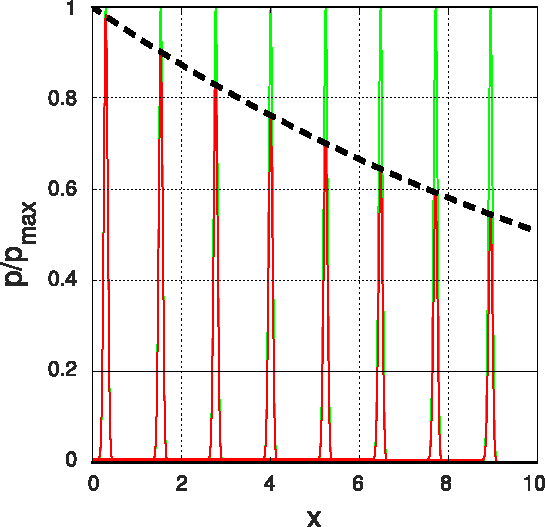
\includegraphics[width=0.9\linewidth]{problem2_article.pdf}
\caption{Результаты из~\cite{boileau:2015}}\label{fig:prob2_a}
\end{subfigure}%
\begin{subfigure}{0.5\linewidth}\centering
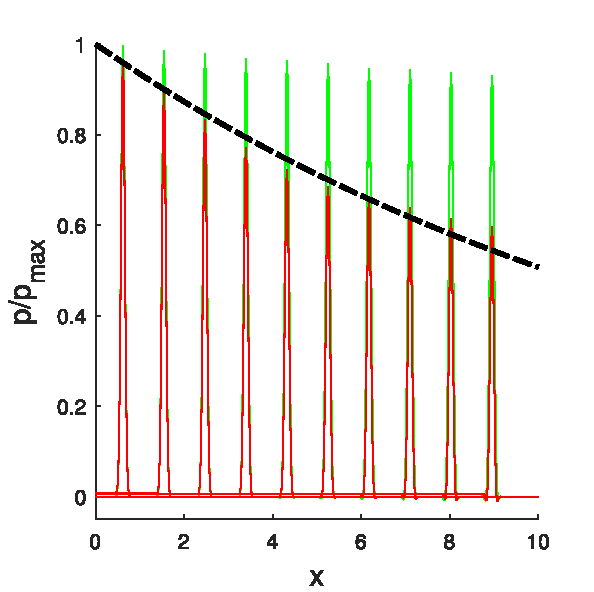
\includegraphics[width=0.9\linewidth]{problem2_theta05.pdf}
\caption{$\theta=0.5$}\label{fig:prob2_b}
\end{subfigure} \\
\hfill \\
\begin{subfigure}{0.5\linewidth}\centering
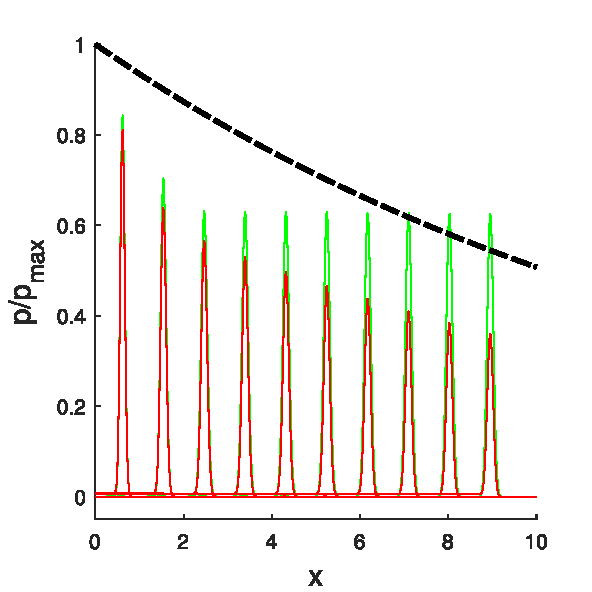
\includegraphics[width=0.9\linewidth]{problem2_theta1.pdf}
\caption{$\theta=1$}\label{fig:prob2_c}
\end{subfigure}%
\begin{subfigure}{0.5\linewidth}\centering
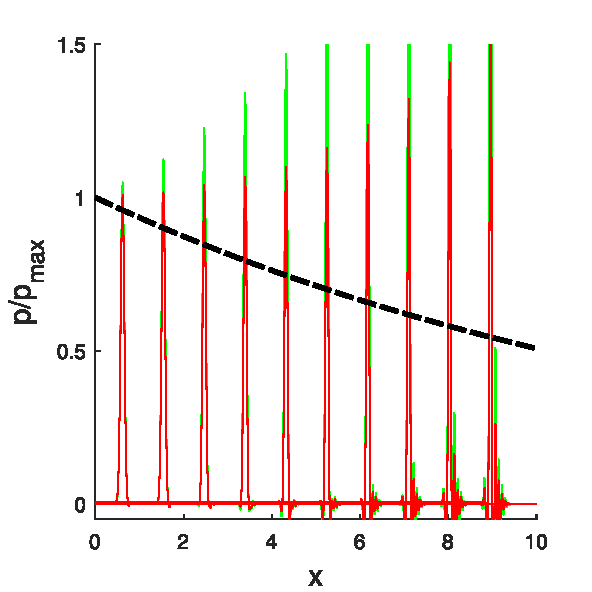
\includegraphics[width=0.9\linewidth]{problem2_theta0.pdf}
\caption{$\theta=0$}\label{fig:prob2_d}
\end{subfigure}%
\caption{Положение скачка давления в различные моменты времени: зелёная линия -- расчёт без вязкости, красная линия -- расчёт с $\mu$=4мПа,
чёрный пунктир -- падение пика давления с продвижением фронта \cref{eq:p_peak_visc}}\label{fig:prob2}
\end{figure}


\subsection{Течение в одиночном сосуде с разрывными свойствами}
%\subsubsection{Сосуд со вставкой}

\begin{figure}[h!]
\begin{subfigure}{0.5\linewidth}\centering
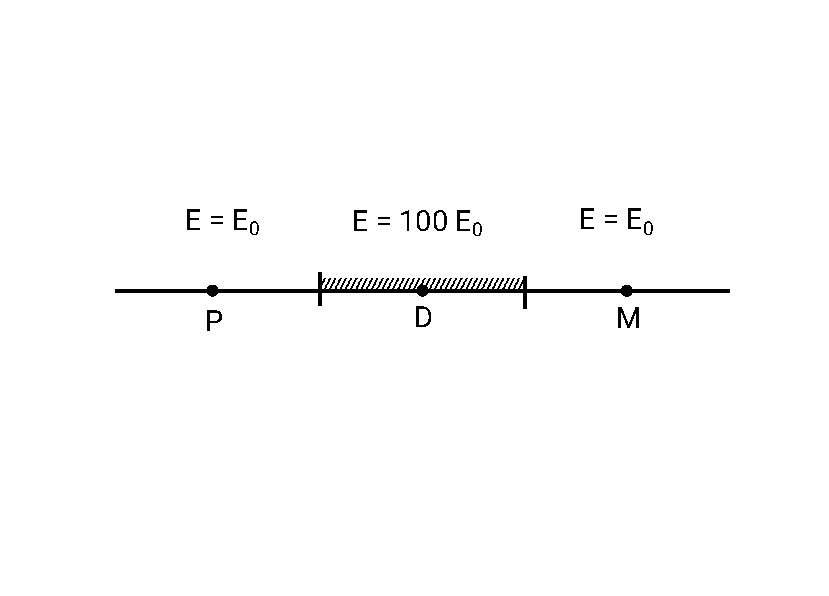
\includegraphics[width=0.9\linewidth]{problem3_def.pdf}
\caption{Cхема сосуда и расположение контрольных точек}\label{fig:prob3_def}
\end{subfigure}%
\begin{subfigure}{0.5\linewidth}\centering
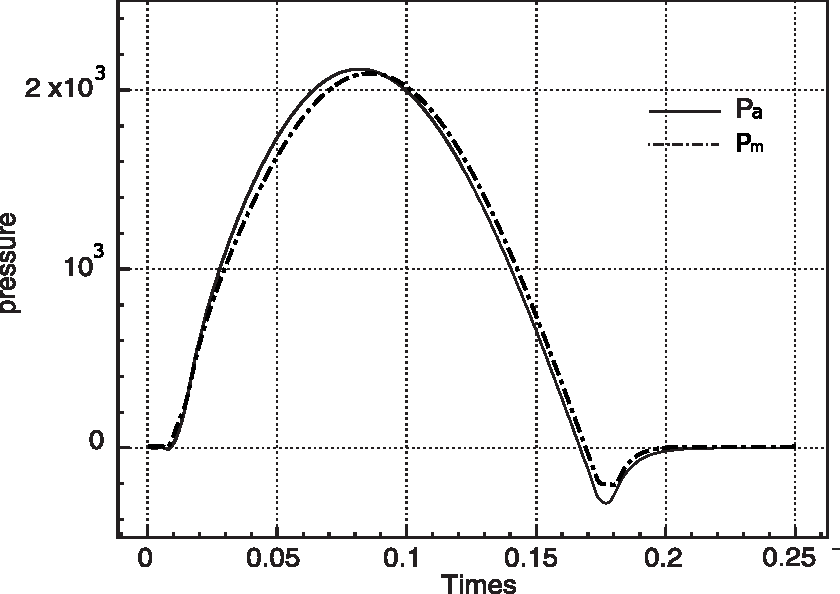
\includegraphics[width=0.9\linewidth]{problem3_P.pdf}
\caption{Контрольная $P$ точка перед вставкой}\label{fig:prob3_a}
\end{subfigure}\\
\par\bigskip % force a bit of vertical whitespace
\begin{subfigure}{0.5\linewidth}\centering
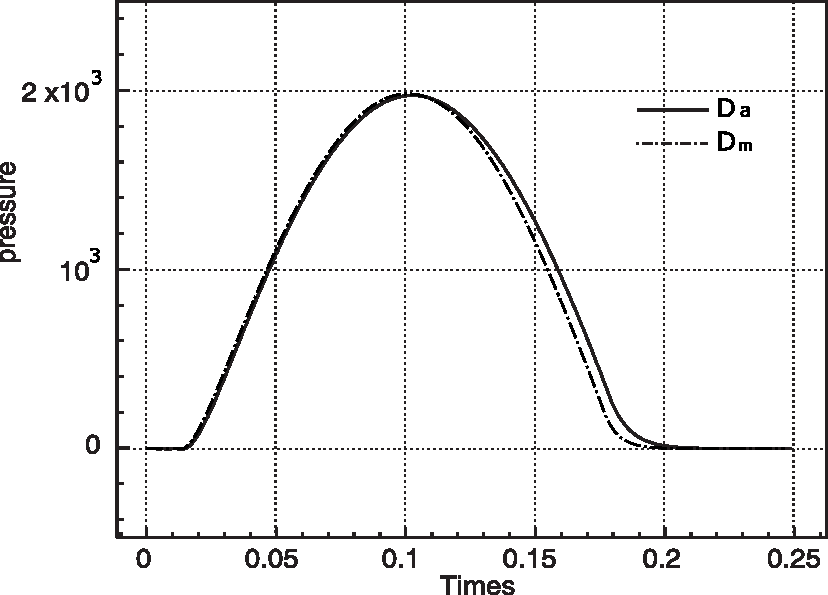
\includegraphics[width=0.9\linewidth]{problem3_D.pdf}
\caption{Контрольная точка $D$ в вставке}\label{fig:prob3_b}
\end{subfigure}%
\begin{subfigure}{0.5\linewidth}\centering
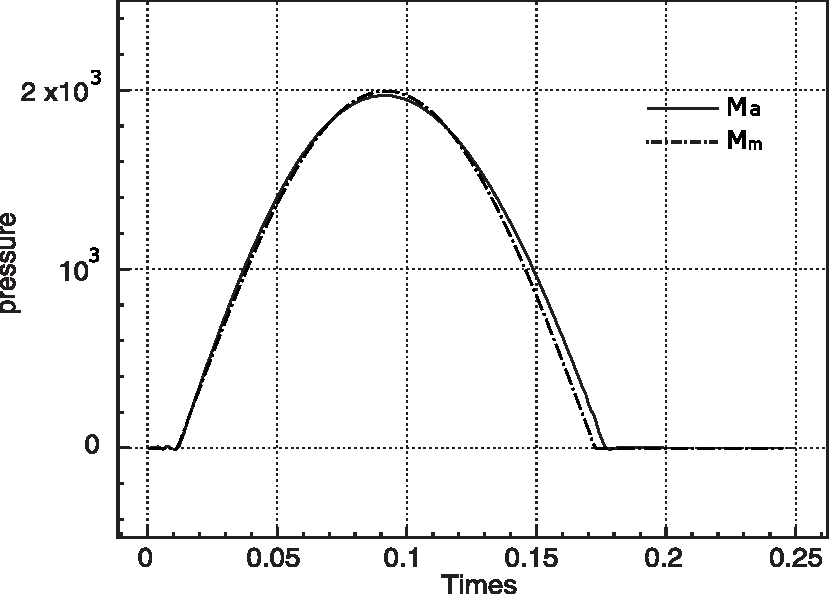
\includegraphics[width=0.9\linewidth]{problem3_M.pdf}
\caption{Контрольная точка $M$ после вставки}\label{fig:prob3_c}
\end{subfigure}%
\caption{Сравнение значения давления в контрольных точках. Сплошная линия -- наш расчёт, пунктирная -- результаты~\cite{Sherwin2003}}\label{fig:prob3}
\end{figure}

В следующем тесте рассмотрим течение в сосуде, имеющим
жёсткую вставку, модуль Юнга в которой на два порядка превышает
значение в остальном сосуде~\cite{Sherwin2003}.
Использовались следующие параметры расчёта
\begin{equation}
\nonumber
\begin{array}{l|c|c}
\text{параметр}  & \text{основной сосуд} & \text{вставка}\\
\hline
\text{длина, м} & 2\times5 & 5\\
\hline
R\text{, м} & \multicolumn{2}{c}{0.5}\\
\hline
E\text{, кПа} & 150 & 15000\\
\hline
h\text{, м} & \multicolumn{2}{c}{1}\\
\hline
\rho\text{, кг/м\textsuperscript{3}} & \multicolumn{2}{c}{1}\\
\hline
\mu\text{, Па с} & \multicolumn{2}{c}{0}\\
\hline
\end{array}
\end{equation}
На входной границе задавалось давление
\begin{equation*}
\nonumber
p(t) = \begin{cases}
2000\sin(2\pi t/T), \quad &t \leq T/2,\\
0, \quad  & t > T/2
\end{cases}
\end{equation*}
со значением периода $T=0.33$.

В результате скорость распространения возмущений в основной части
канала составляла $c_0\approx450$, а во вставки была больше на порядок.
Расчёт проводился при выборе $\dx = 0.5$, $\dt = \dx 2\cdot10^{-5} = 10^{-5}$. Такой
выбор обеспечивал $\CFL=0.1$ для максимального $c_0$.

Результирующие значение давления в контрольных точках сосуда
представлены на рис.~\ref{fig:prob3} в сравнении с данными~\cite{Sherwin2003}.
Наблюдается удовлетворительное совпадение полученных кривых.

%В приведённом примере характерная длина волны $c_0\timesT/2\approx70$
%была много больше, чем длина области расчёта, однако
%по приведённым графикам можно сделать вывод
Можно отметить, что через контрольную точку $M$ проходит
ровно одна поступательная волна давления, о чём свидетельствует
резкие границы у кривых, приведённых на рис.~\ref{fig:prob3_c}.
Через точки $P$ и $D$ помимо основной поступательной проходят несколько отражённых волн,
поэтому правая граница волны на рисунках~\ref{fig:prob3_a},~\ref{fig:prob3_b}
имеет заметные искажения.


%\subsubsection{Влияние смены свойств стенок сосуда на решение задачи}
%TODO

\subsection{Течение в сосуде с разветвлением}
Рассматривается тестовая задача~\cite{Xiu:2007} о течении в разветвлении сосудов.
Расчётные свойства сосудов до разветвления (сосуд 1) и после разветвления (сосуды 2)
представлены ниже

\begin{equation}
\nonumber
\begin{array}{l|c|c}
\text{параметр}  & \text{сосуд 1} & \text{сосуды 2}\\
\hline
\text{длина, м} & 0.2 & 0.2\\
\hline
R\text{, мм} & 5.0 & 5.0/\sqrt{6}\\
\hline
E\text{, kПа} & 108 & 264.5\\
\hline
h\text{, мм} & \multicolumn{2}{c}{0.1}\\
\hline
\rho\text{, кг/м\textsuperscript{3}} & \multicolumn{2}{c}{1000}\\
\hline
\mu\text{, Па с} & \multicolumn{2}{c}{0}\\
\hline
\end{array}
\end{equation}

\begin{figure}[h!]
\begin{subfigure}{1.0\linewidth}\centering
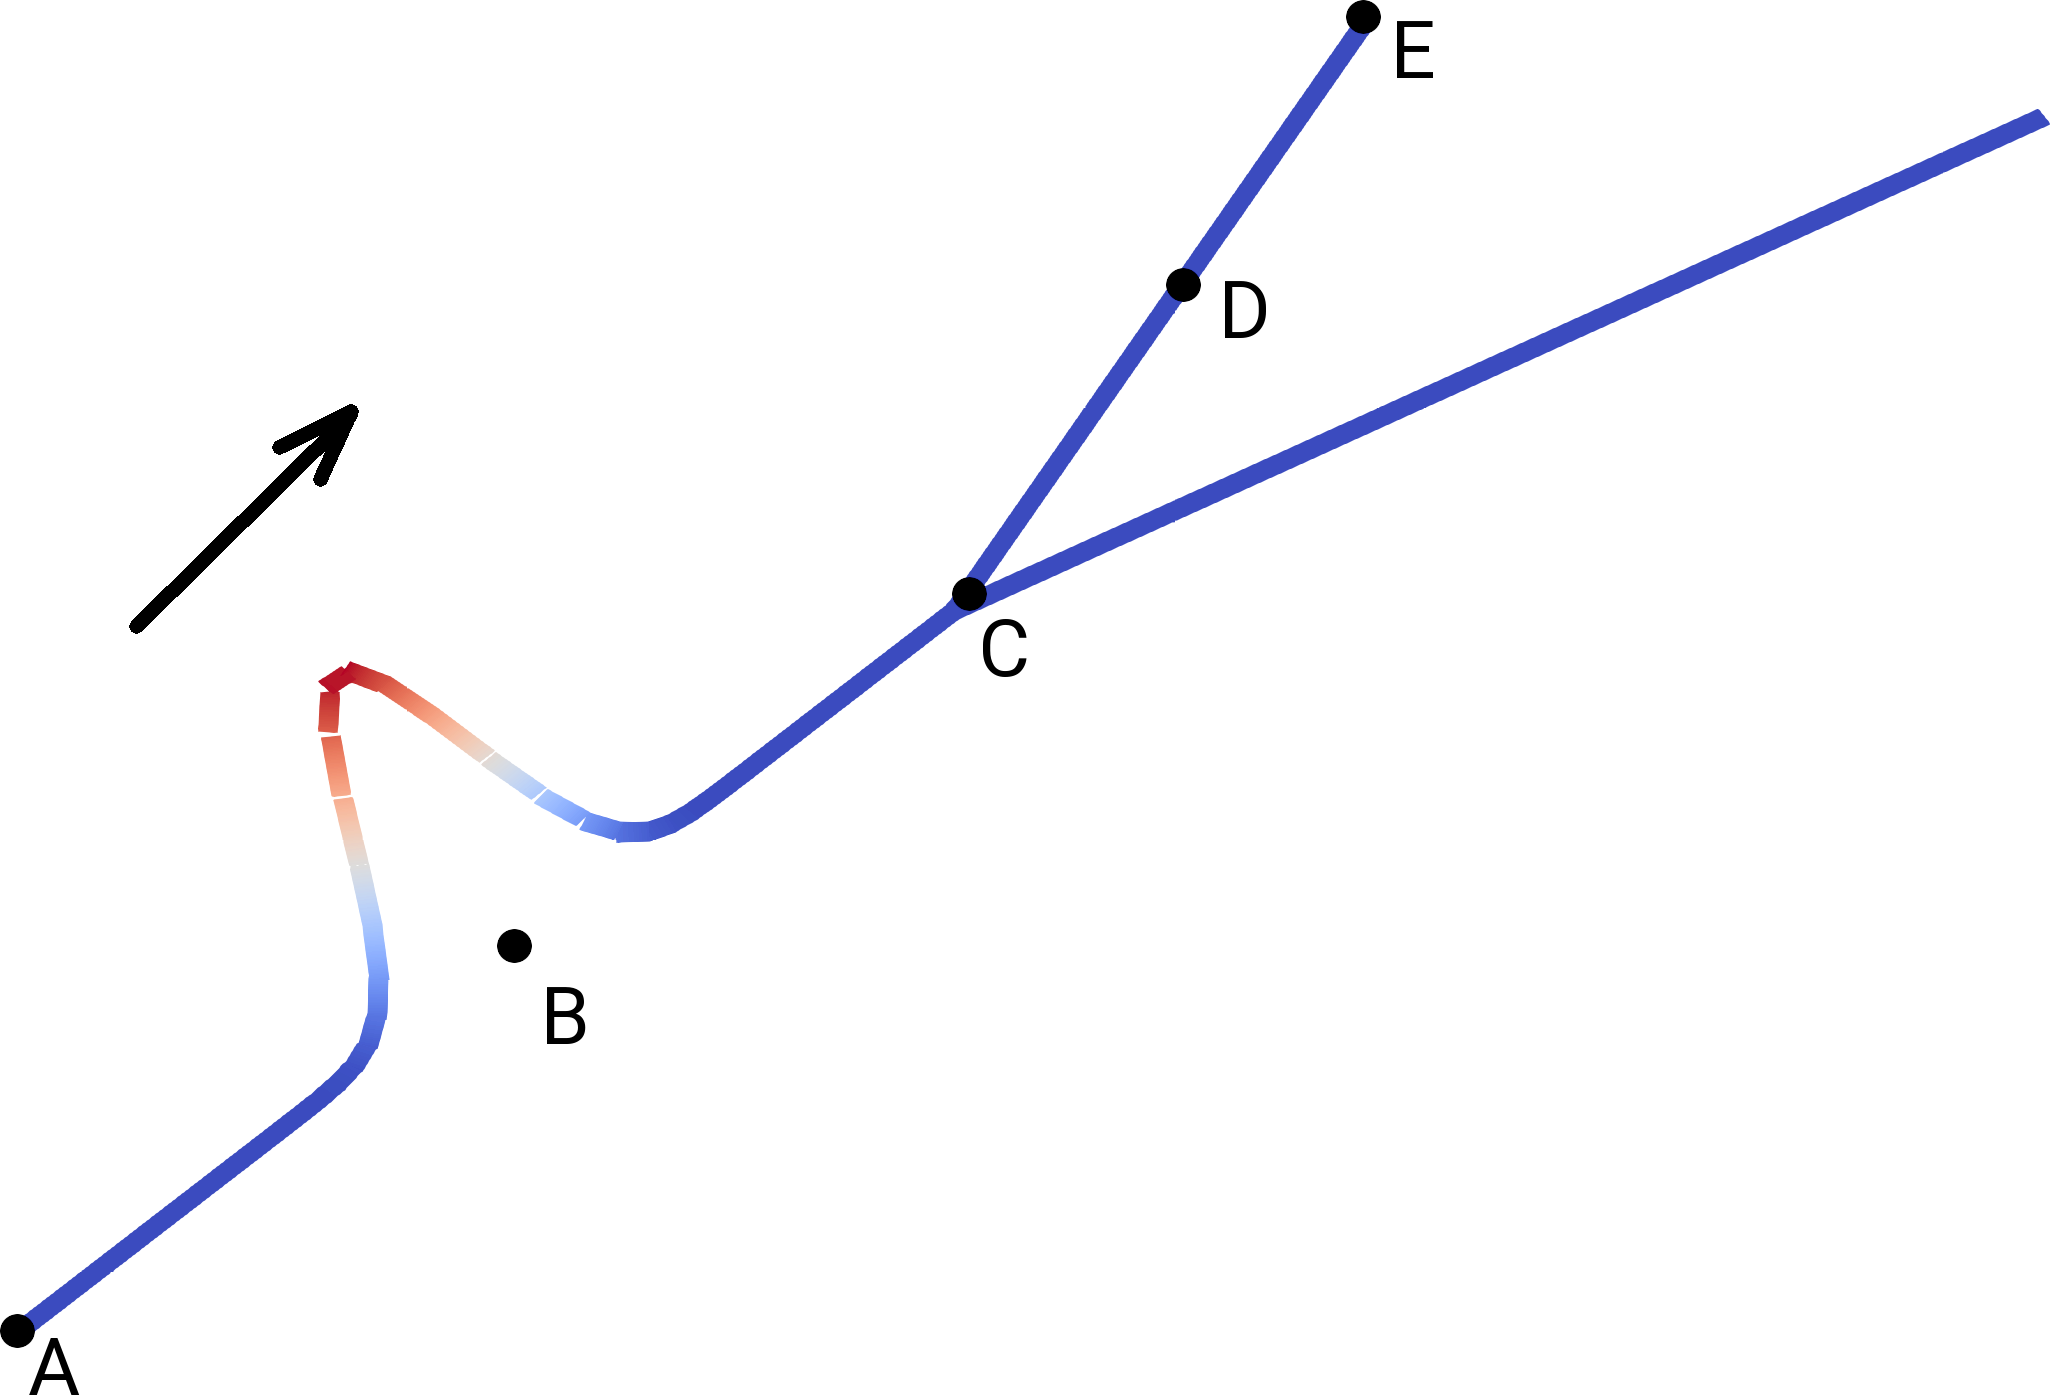
\includegraphics[width=0.4\linewidth]{prob4_time/p0.png}
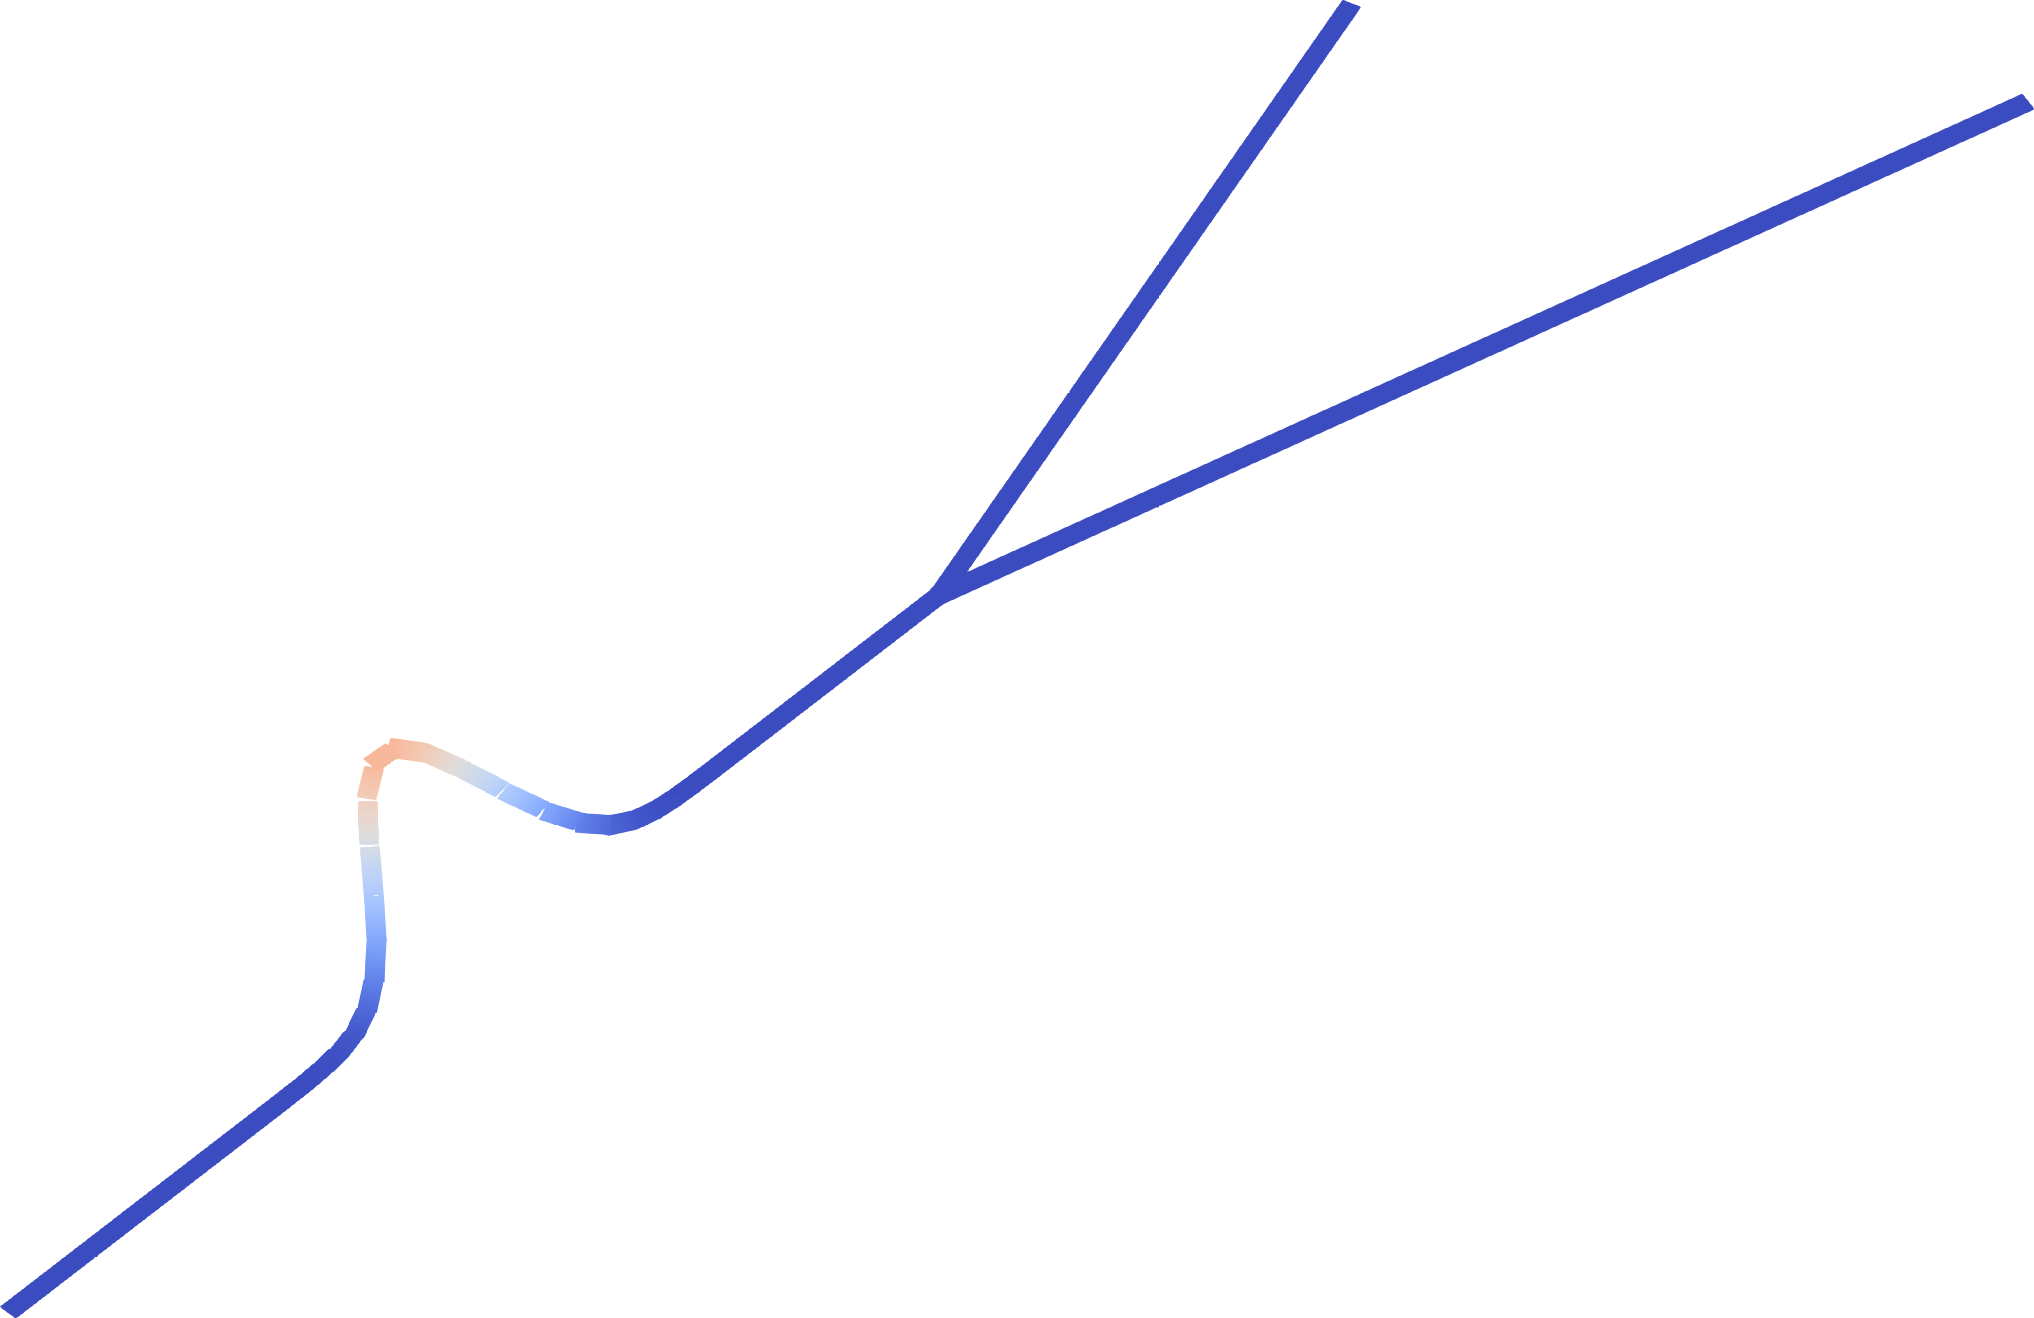
\includegraphics[width=0.4\linewidth]{prob4_time/v0.png}
\caption{$t = 0.13$}\label{fig:prob4_pv_a}
\end{subfigure} \\
\hfill \\
\hfill \\
\begin{subfigure}{1.0\linewidth}\centering
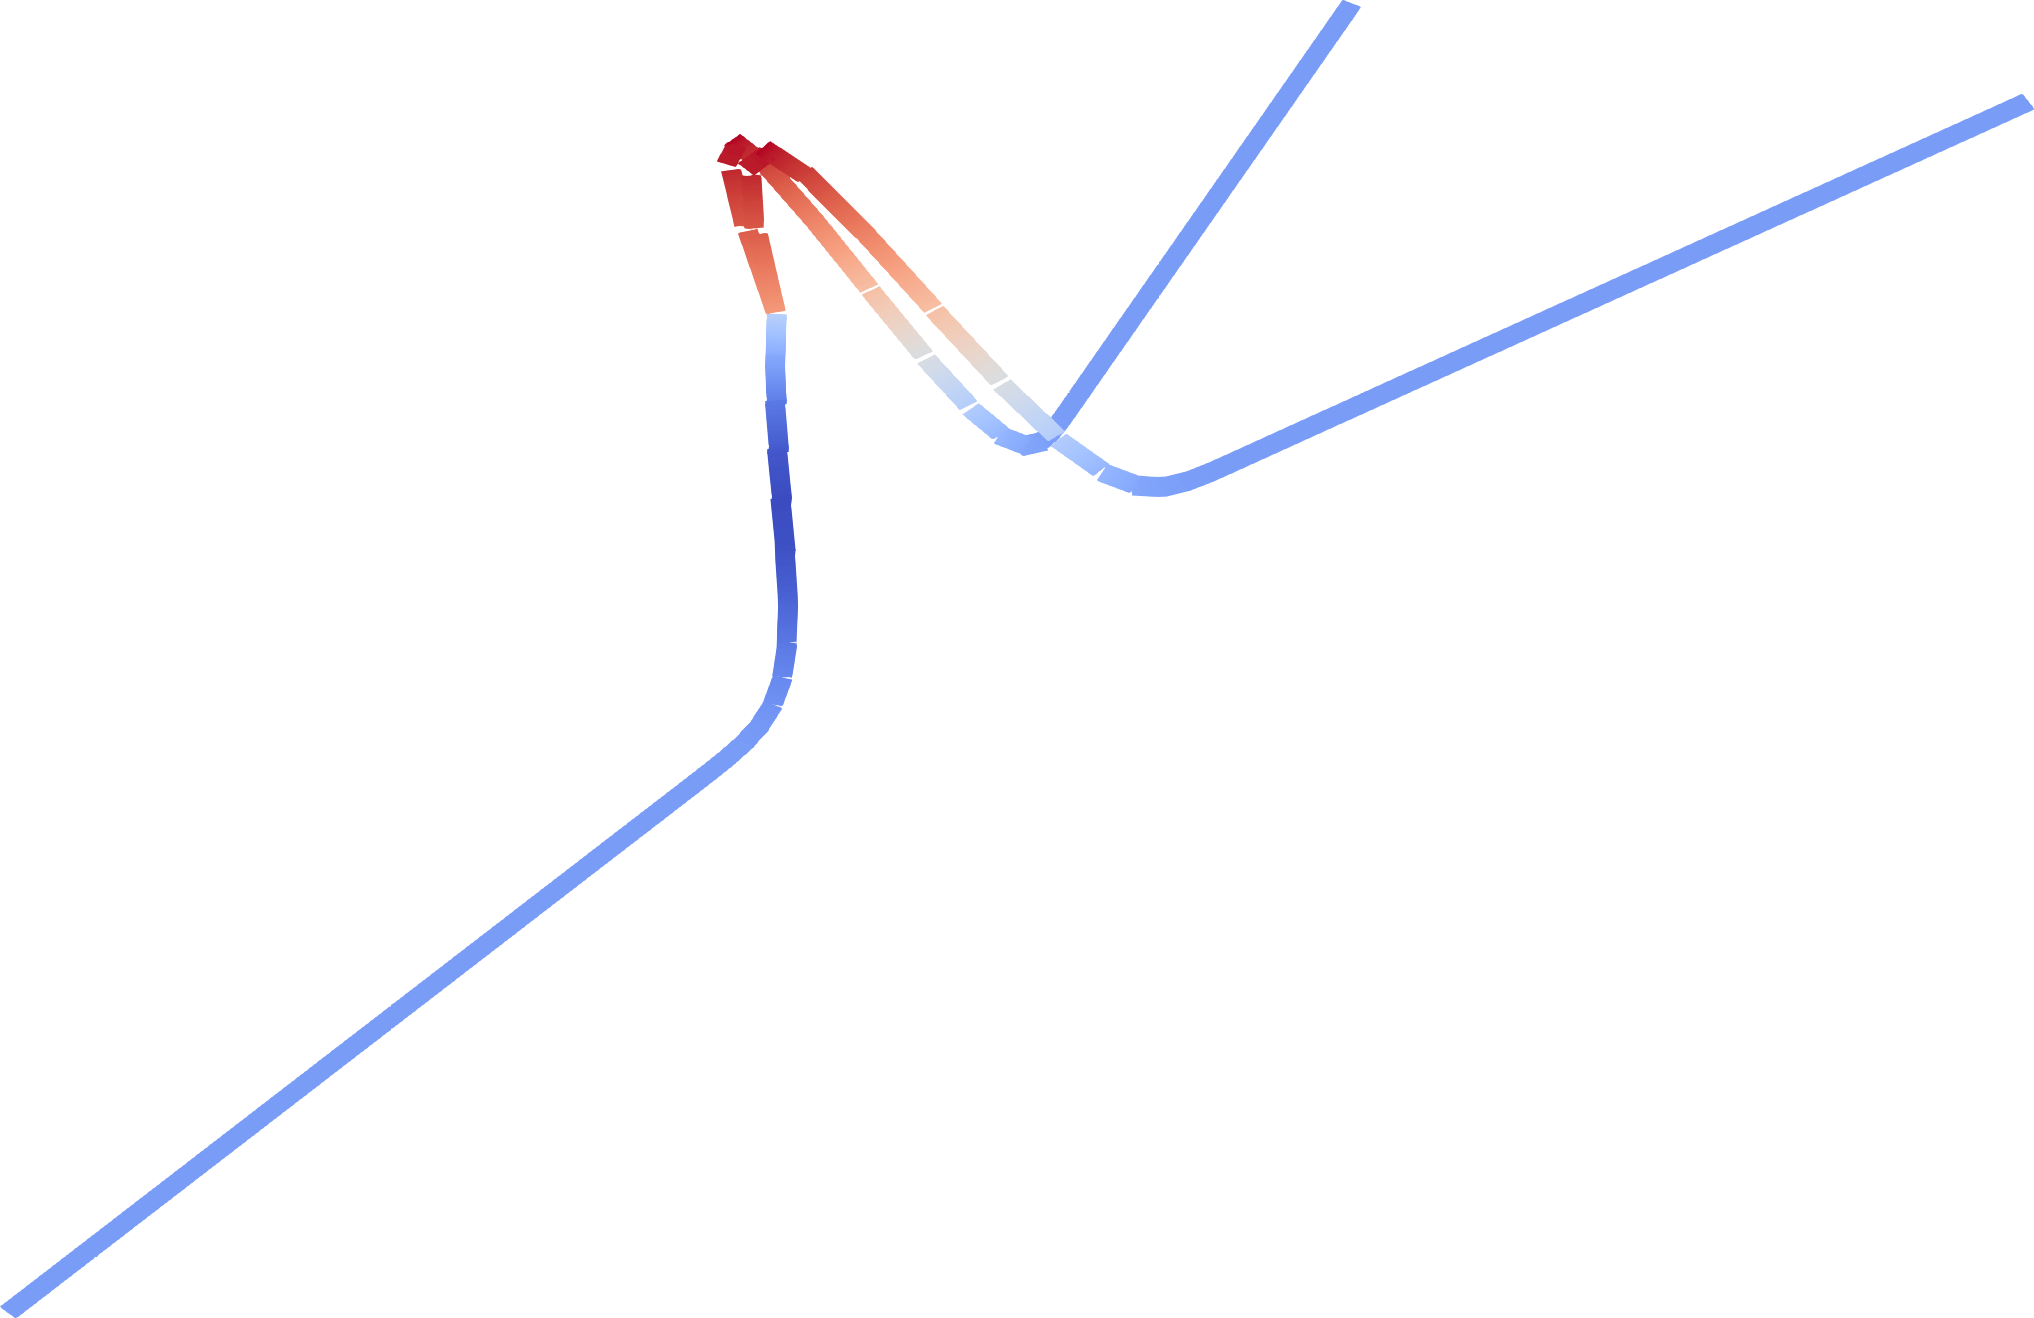
\includegraphics[width=0.4\linewidth]{prob4_time/p1.png}
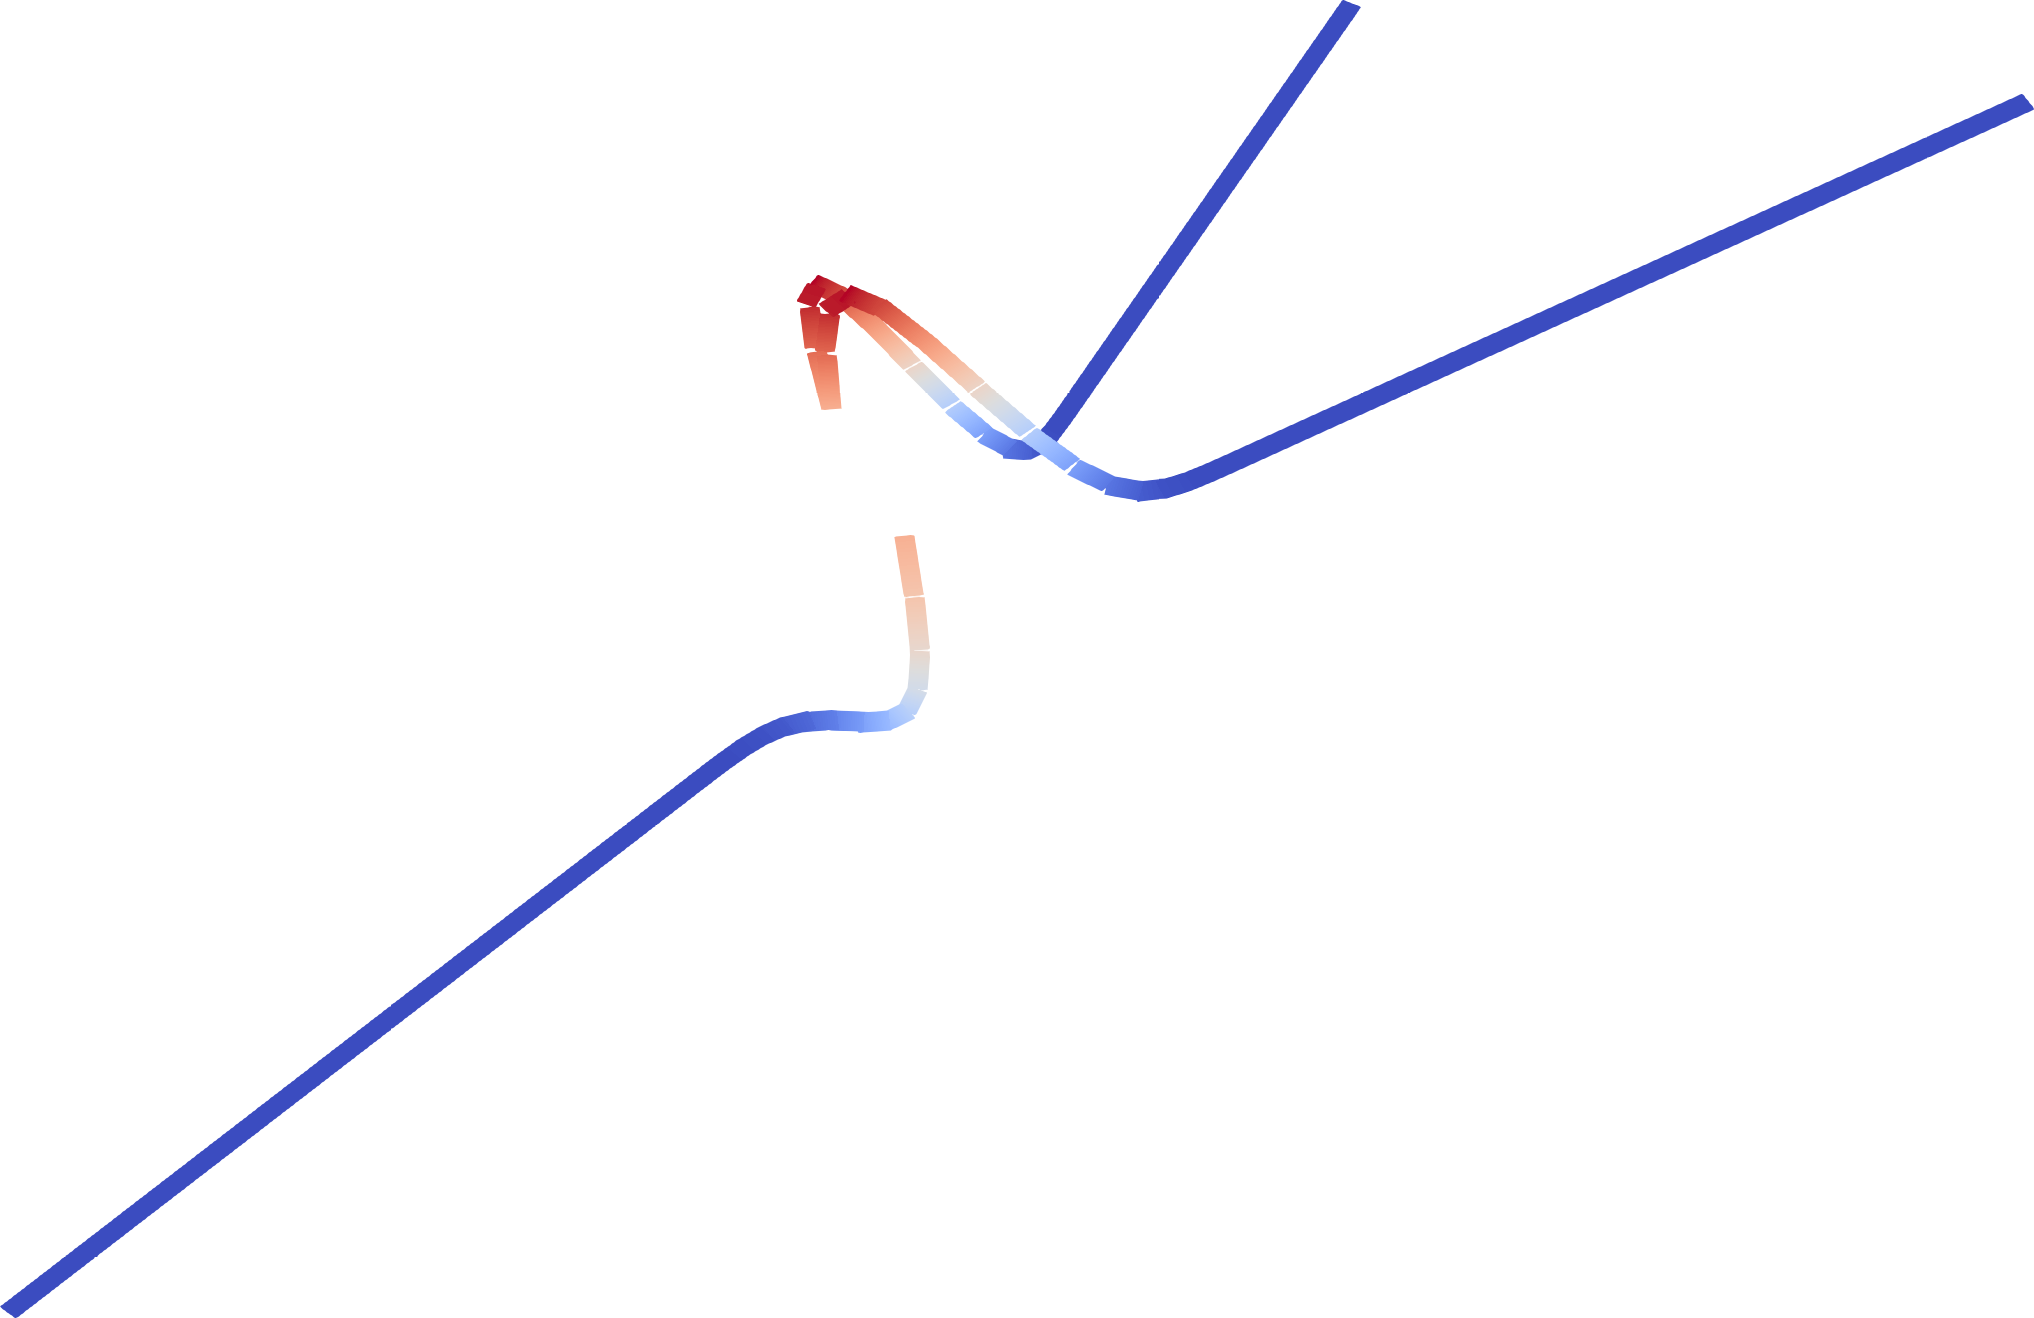
\includegraphics[width=0.4\linewidth]{prob4_time/v1.png}
\caption{$t = 0.22$}\label{fig:prob4_pv_b}
\end{subfigure}\\
\hfill \\
\hfill \\
\begin{subfigure}{1.0\linewidth}\centering
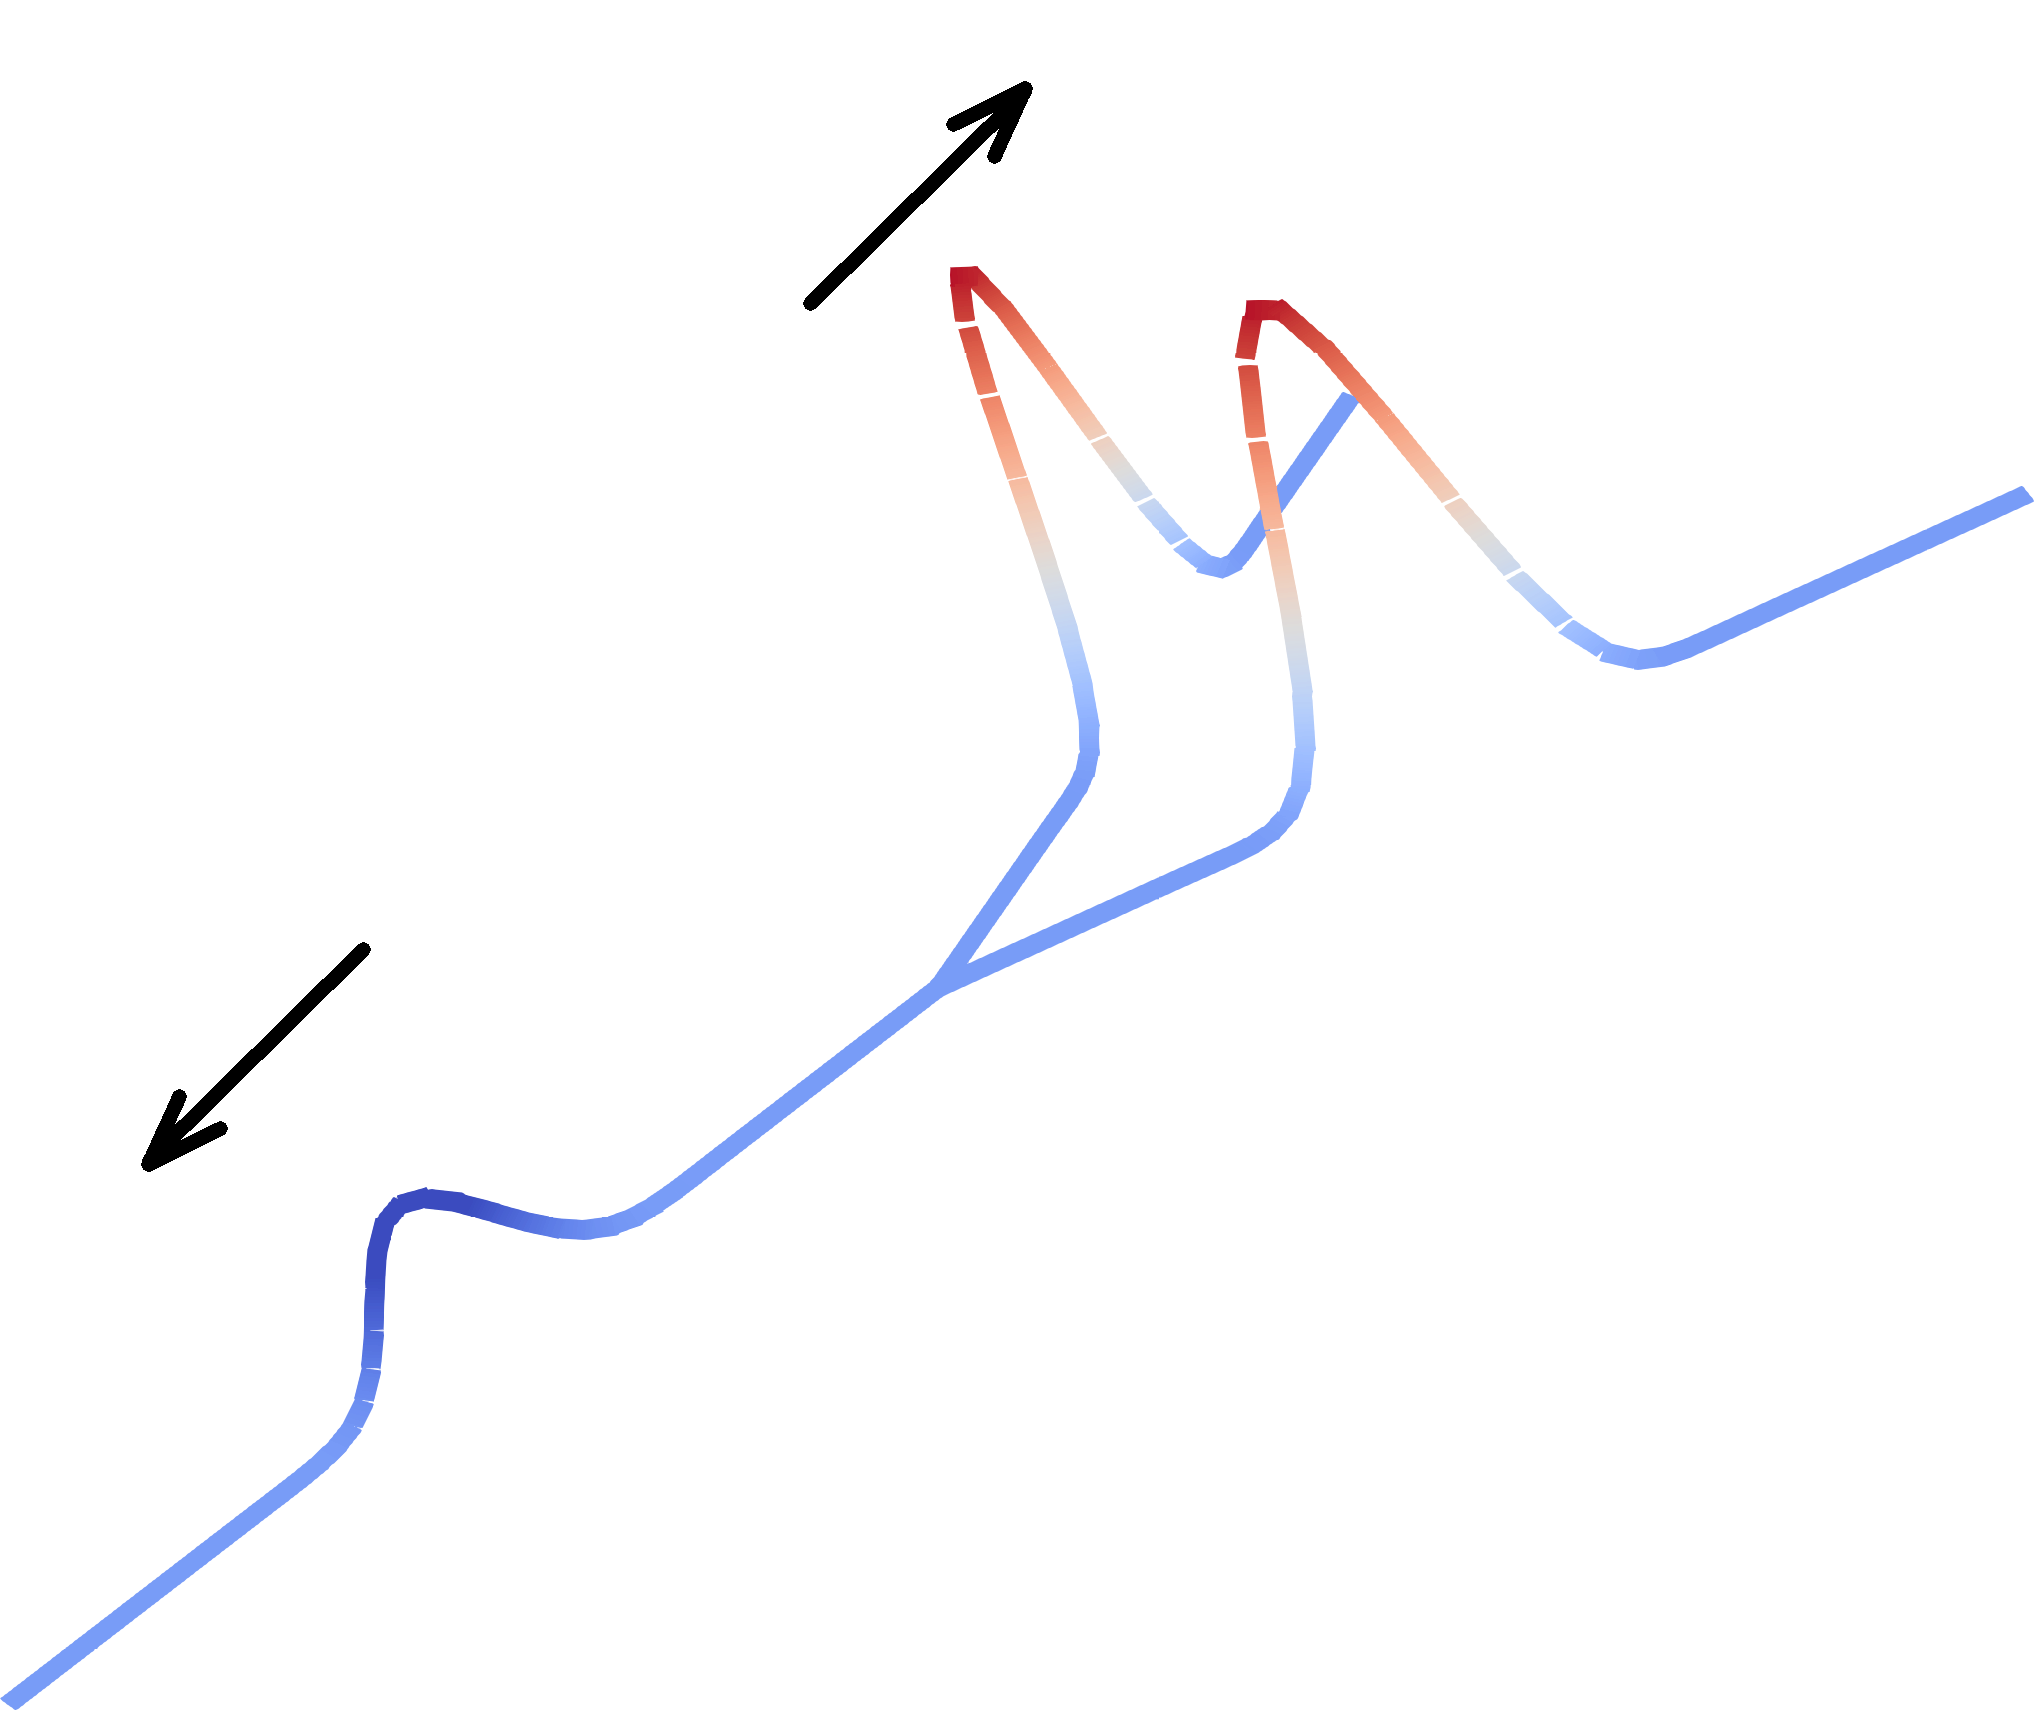
\includegraphics[width=0.4\linewidth]{prob4_time/p2.png}
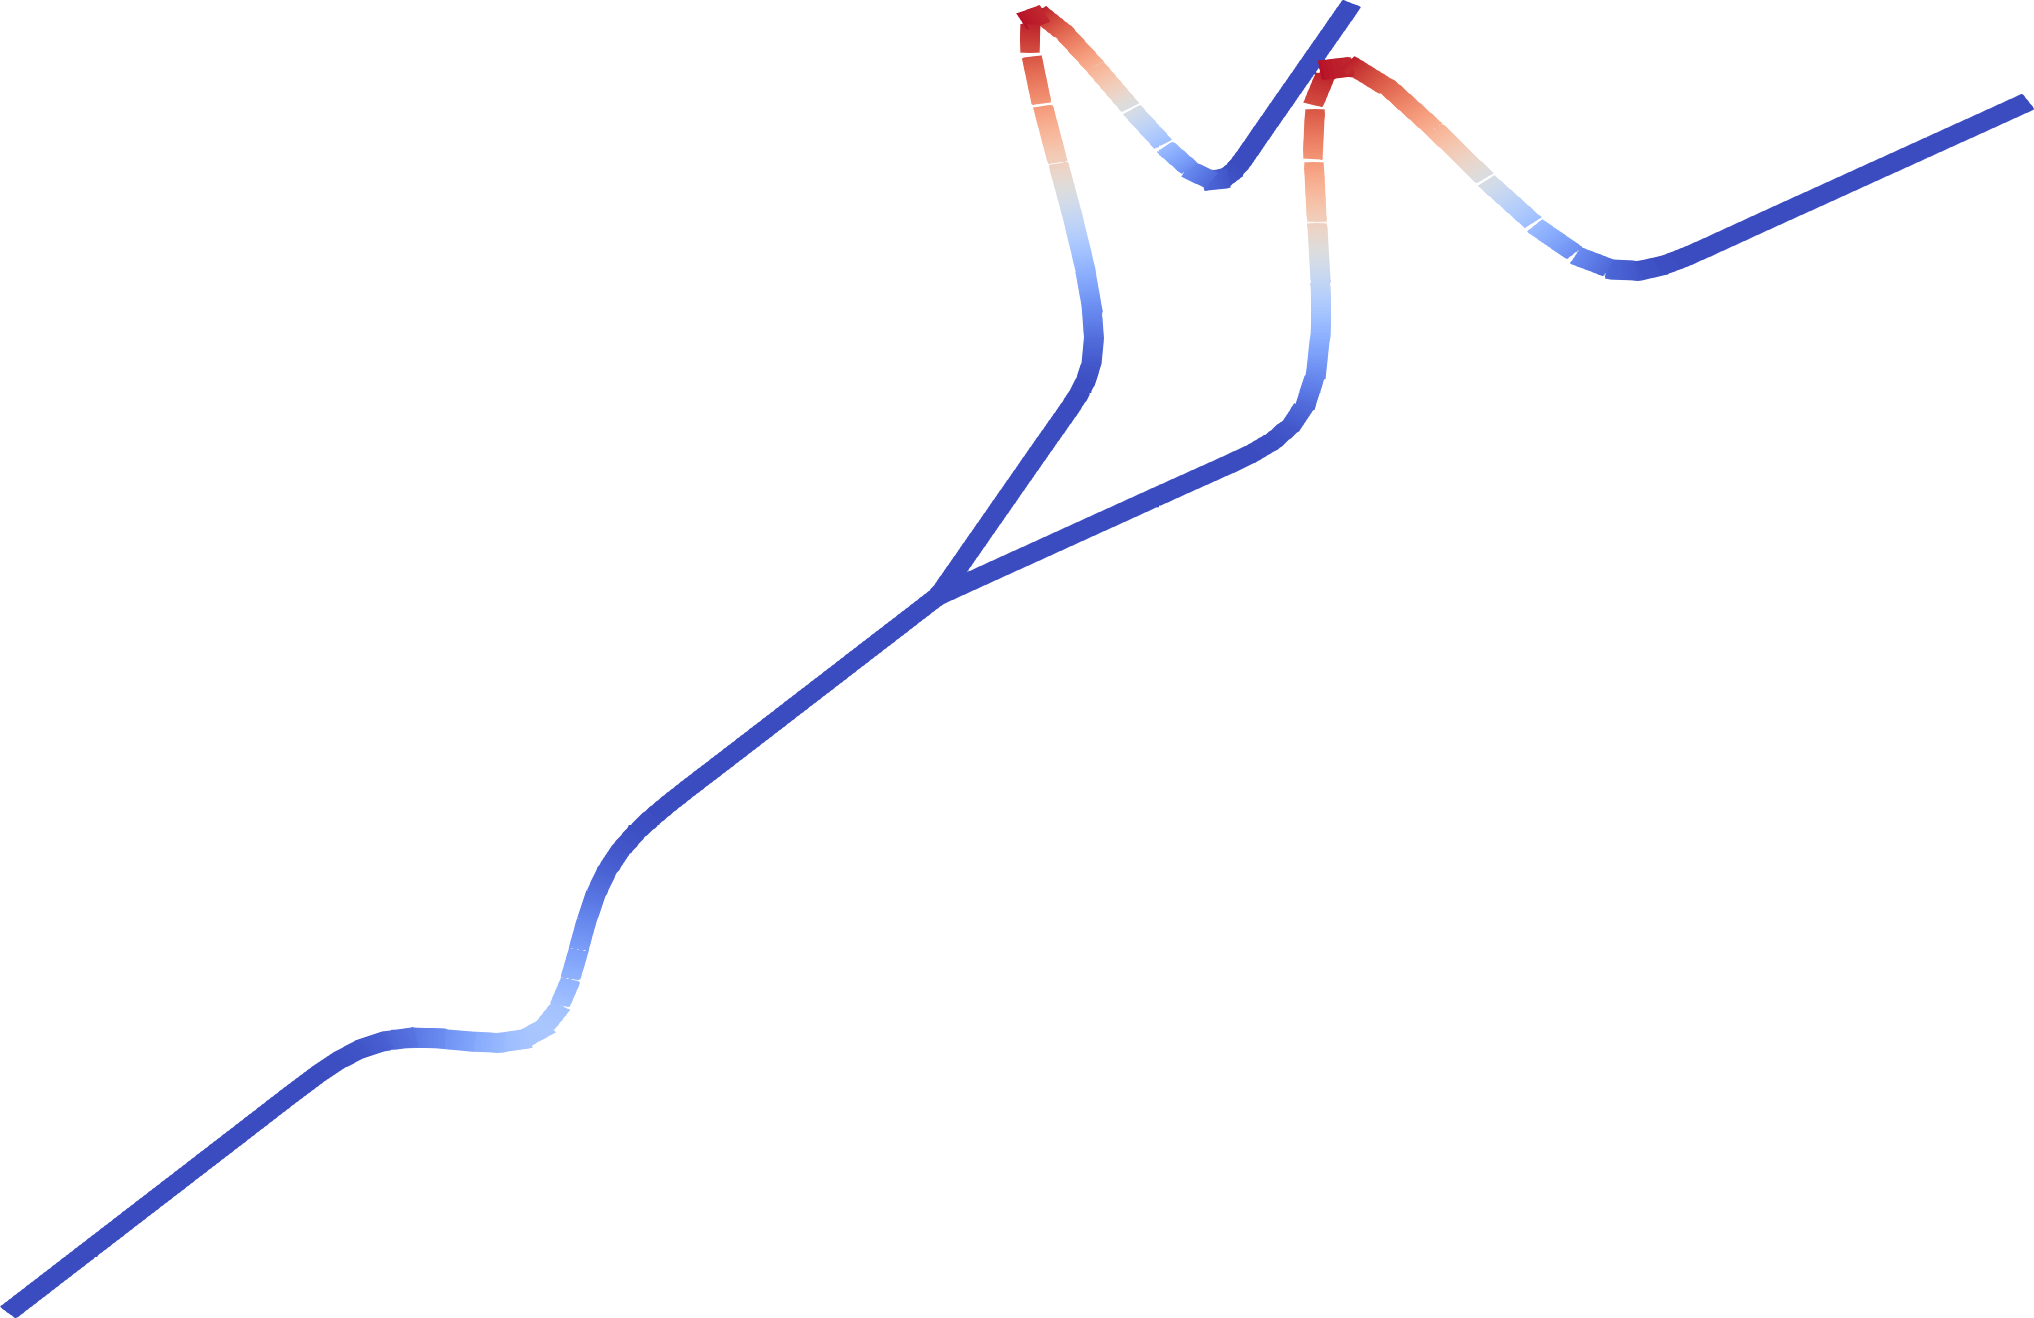
\includegraphics[width=0.4\linewidth]{prob4_time/v2.png}
\caption{$t=0.3$}\label{fig:prob4_pv_c}
\end{subfigure}\\
\caption{Значение давления (слева) и скорости (справа) на различные моменты времени}\label{fig:prob4_pv}
\end{figure}

\begin{figure}[h!]
\begin{subfigure}{1.0\linewidth}\centering
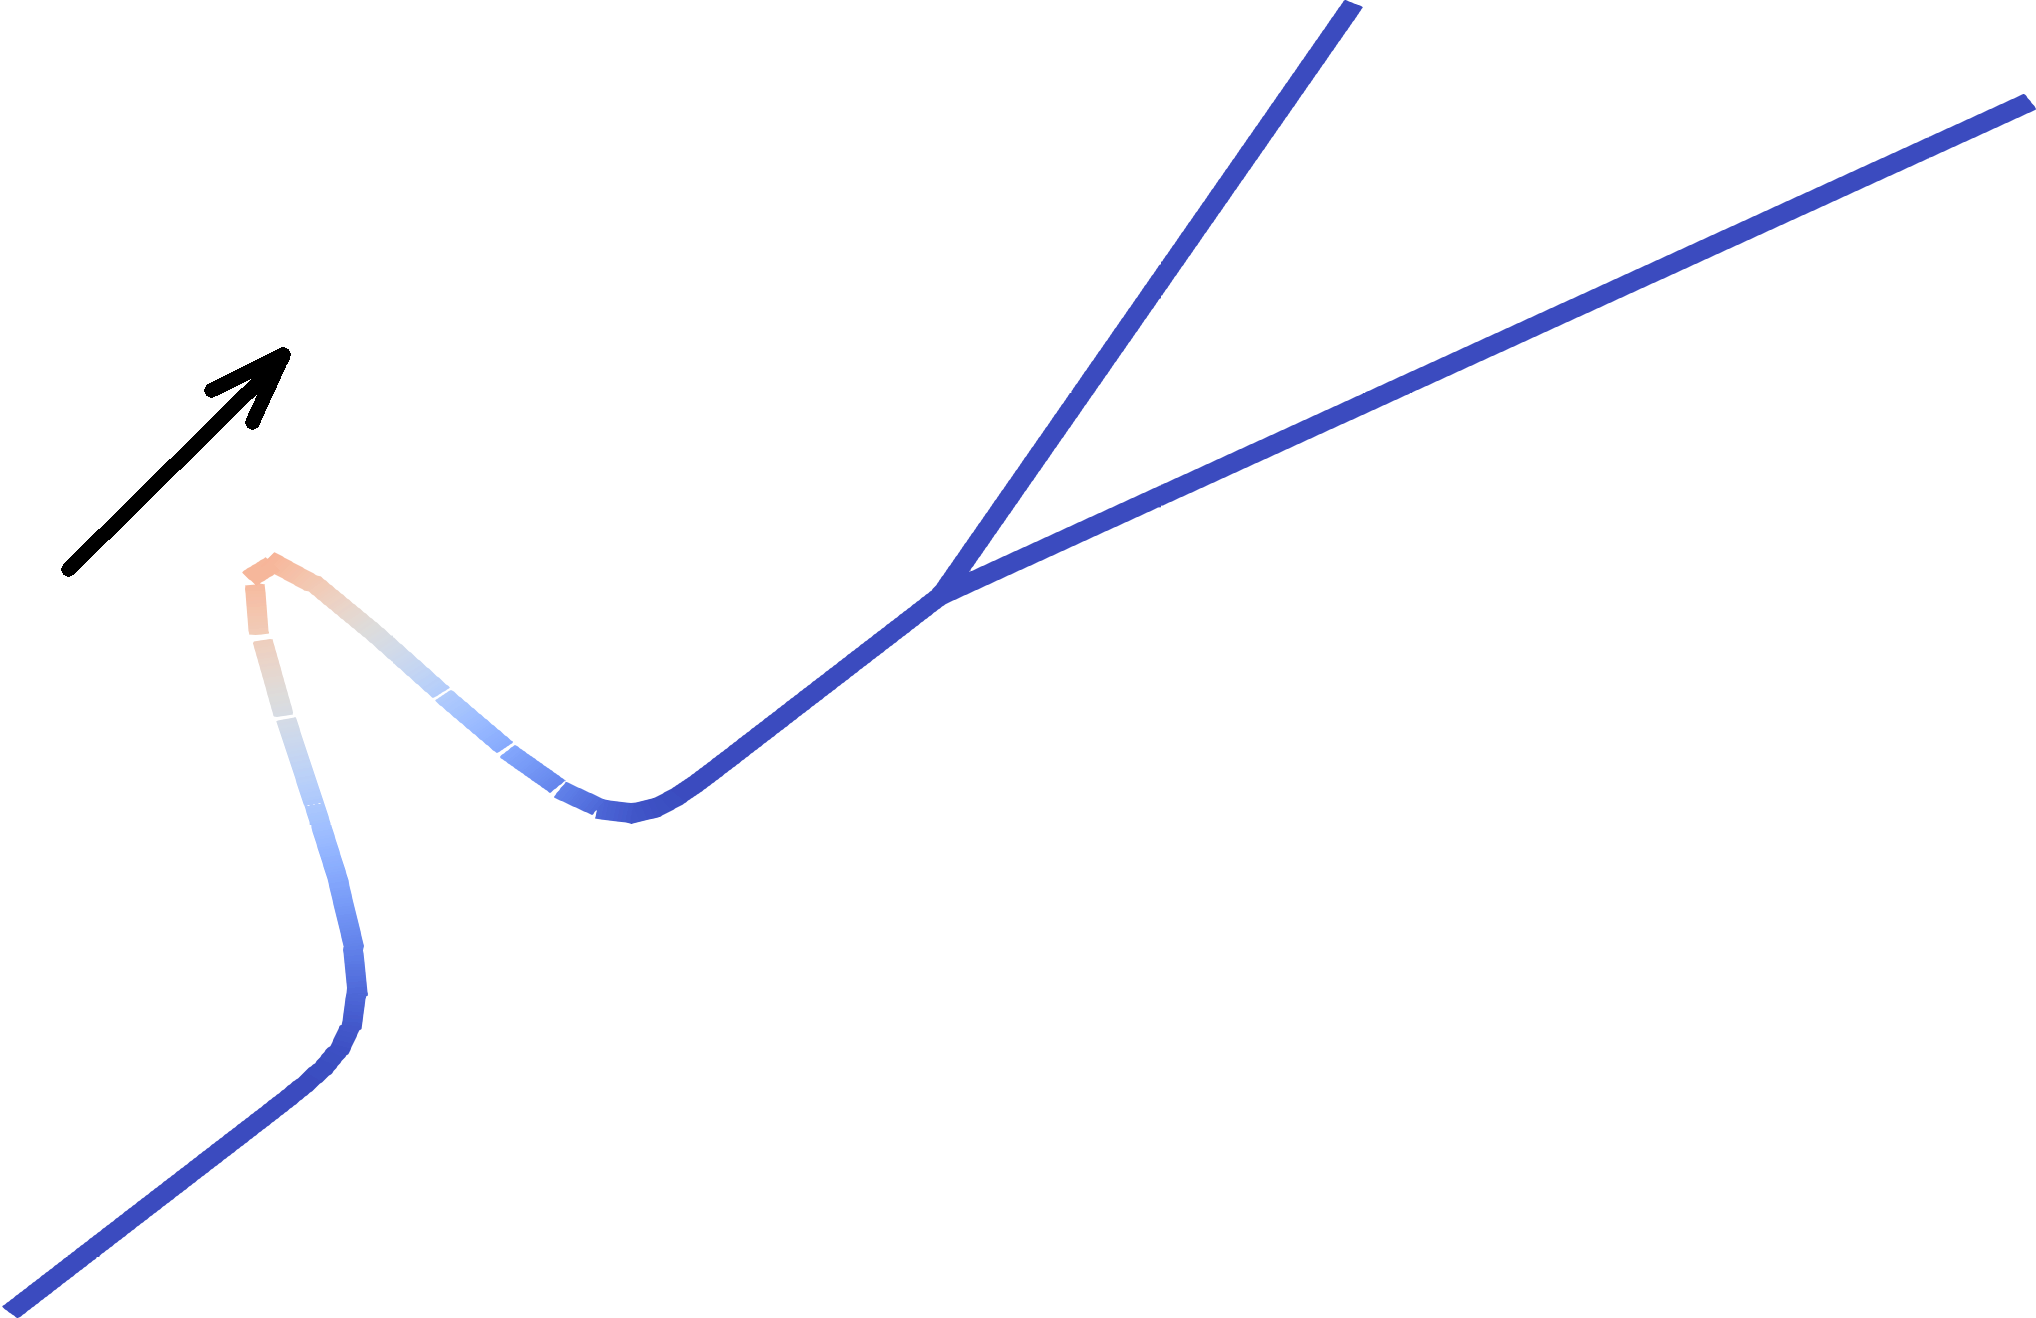
\includegraphics[width=0.4\linewidth]{prob4_time/w1_0.png}
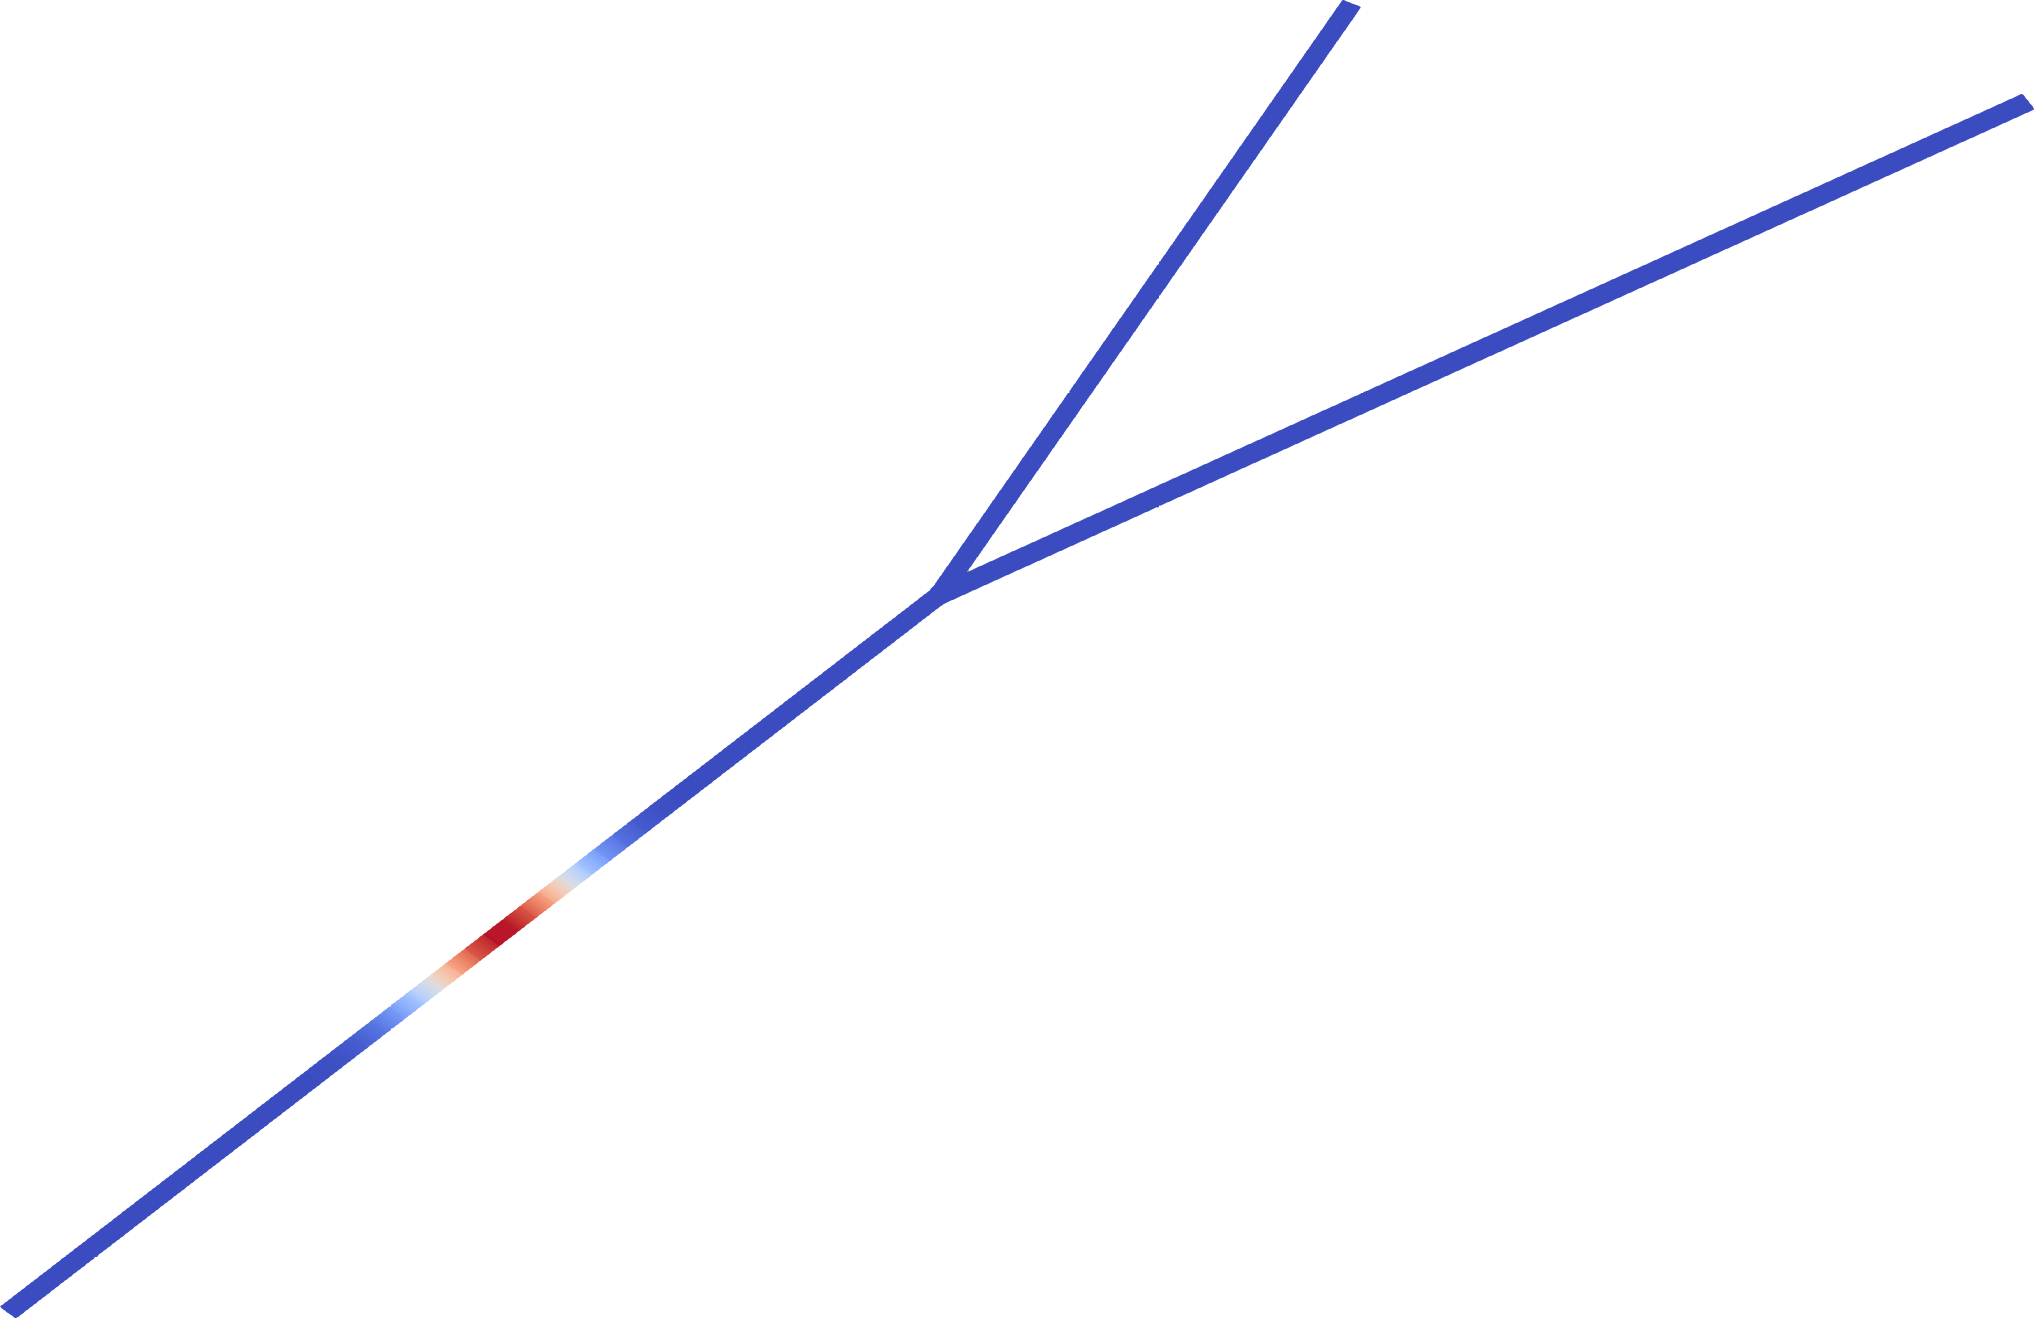
\includegraphics[width=0.4\linewidth]{prob4_time/w2_0.png}
\caption{$t = 0.13$}\label{fig:prob4_w12_a}
\end{subfigure} \\
\hfill \\
\hfill \\
\begin{subfigure}{1.0\linewidth}\centering
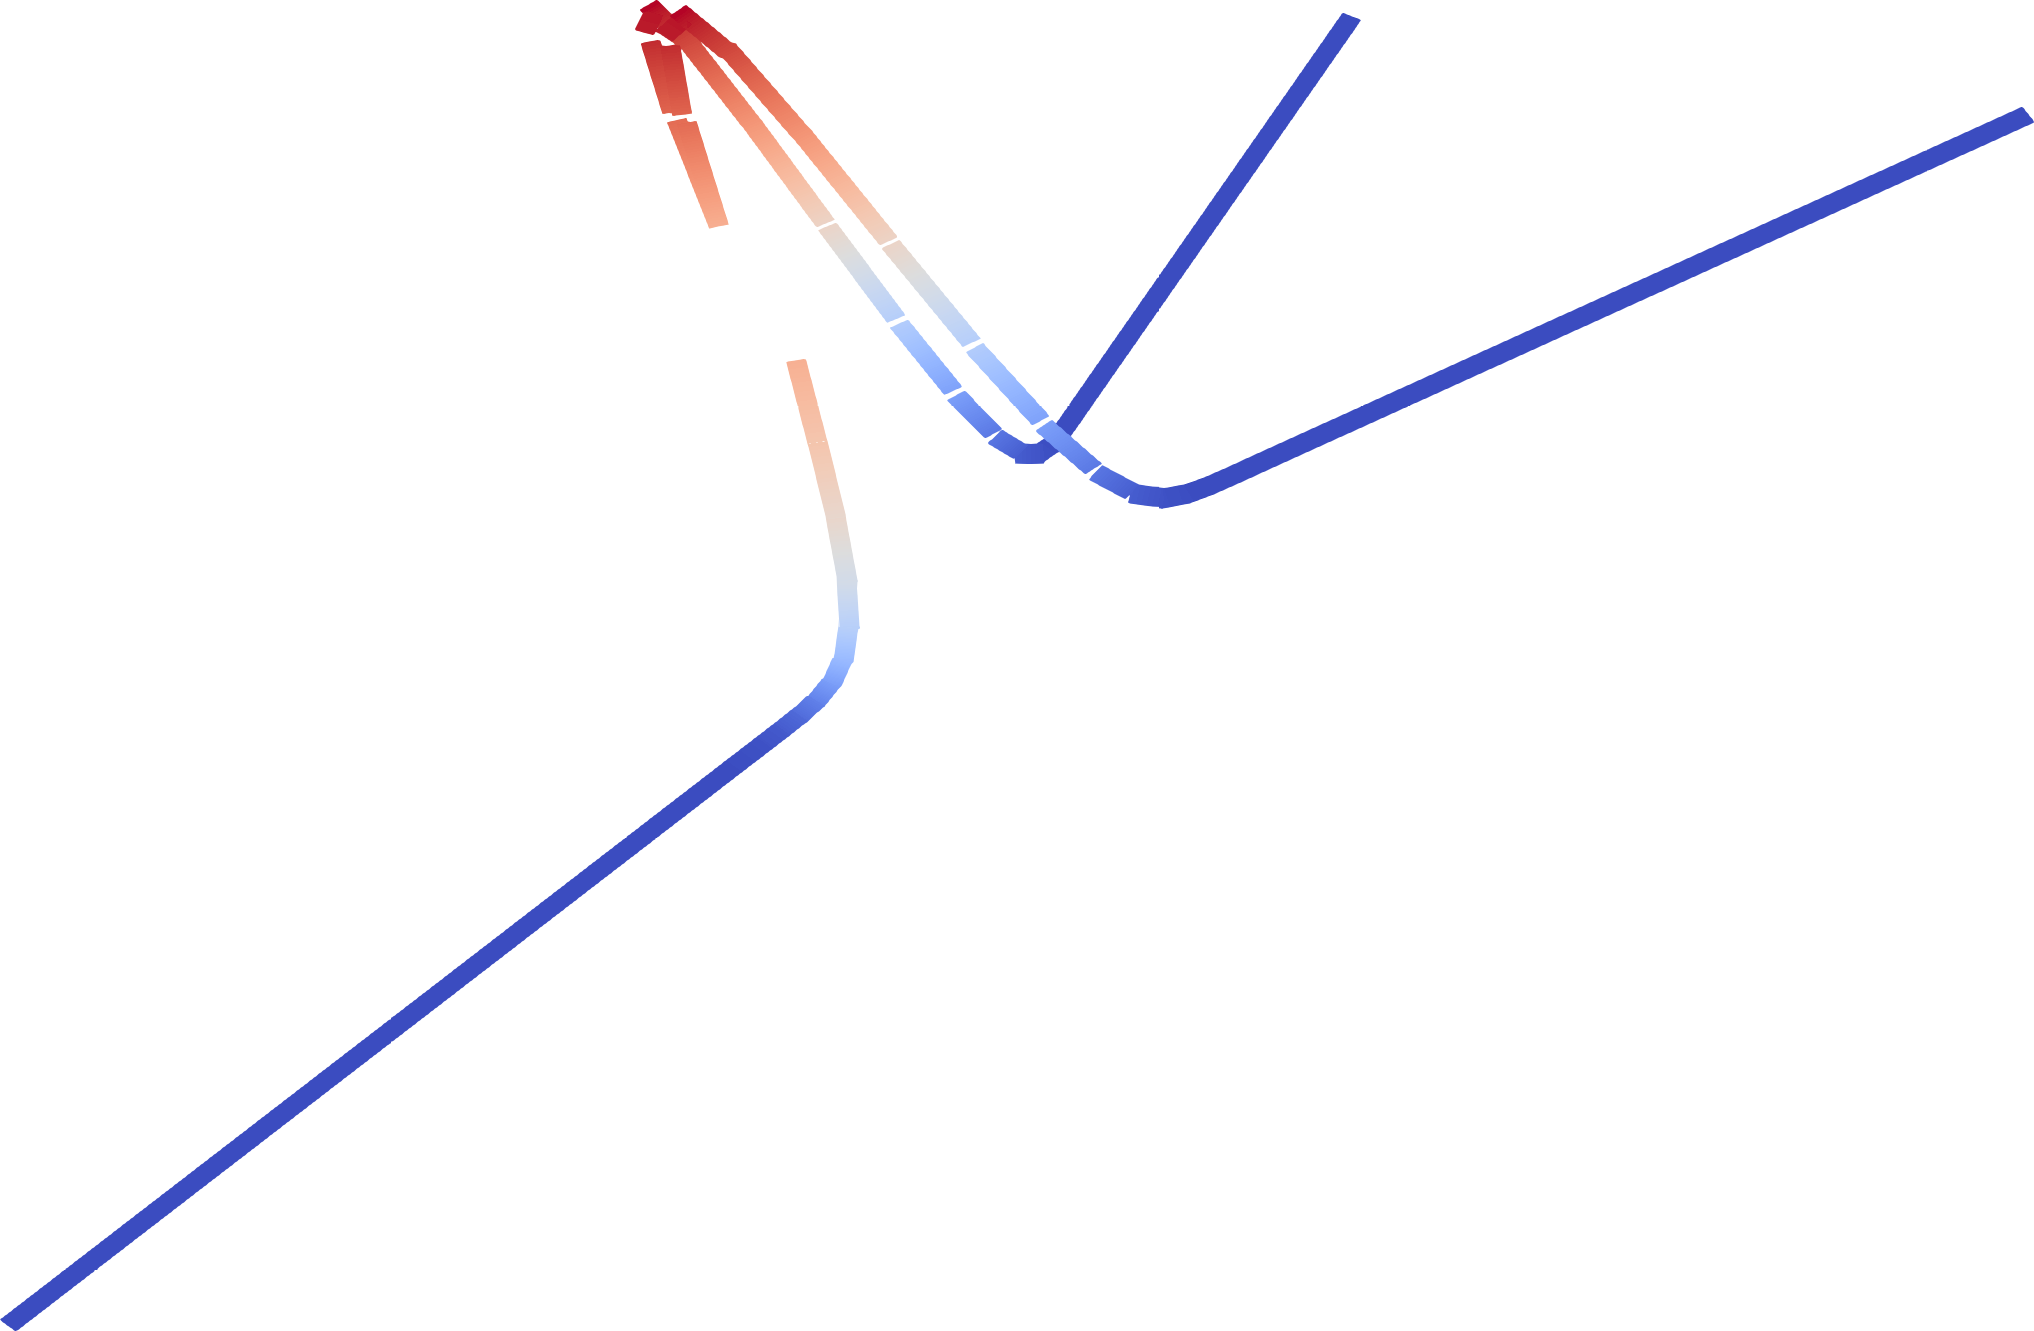
\includegraphics[width=0.4\linewidth]{prob4_time/w1_1.png}
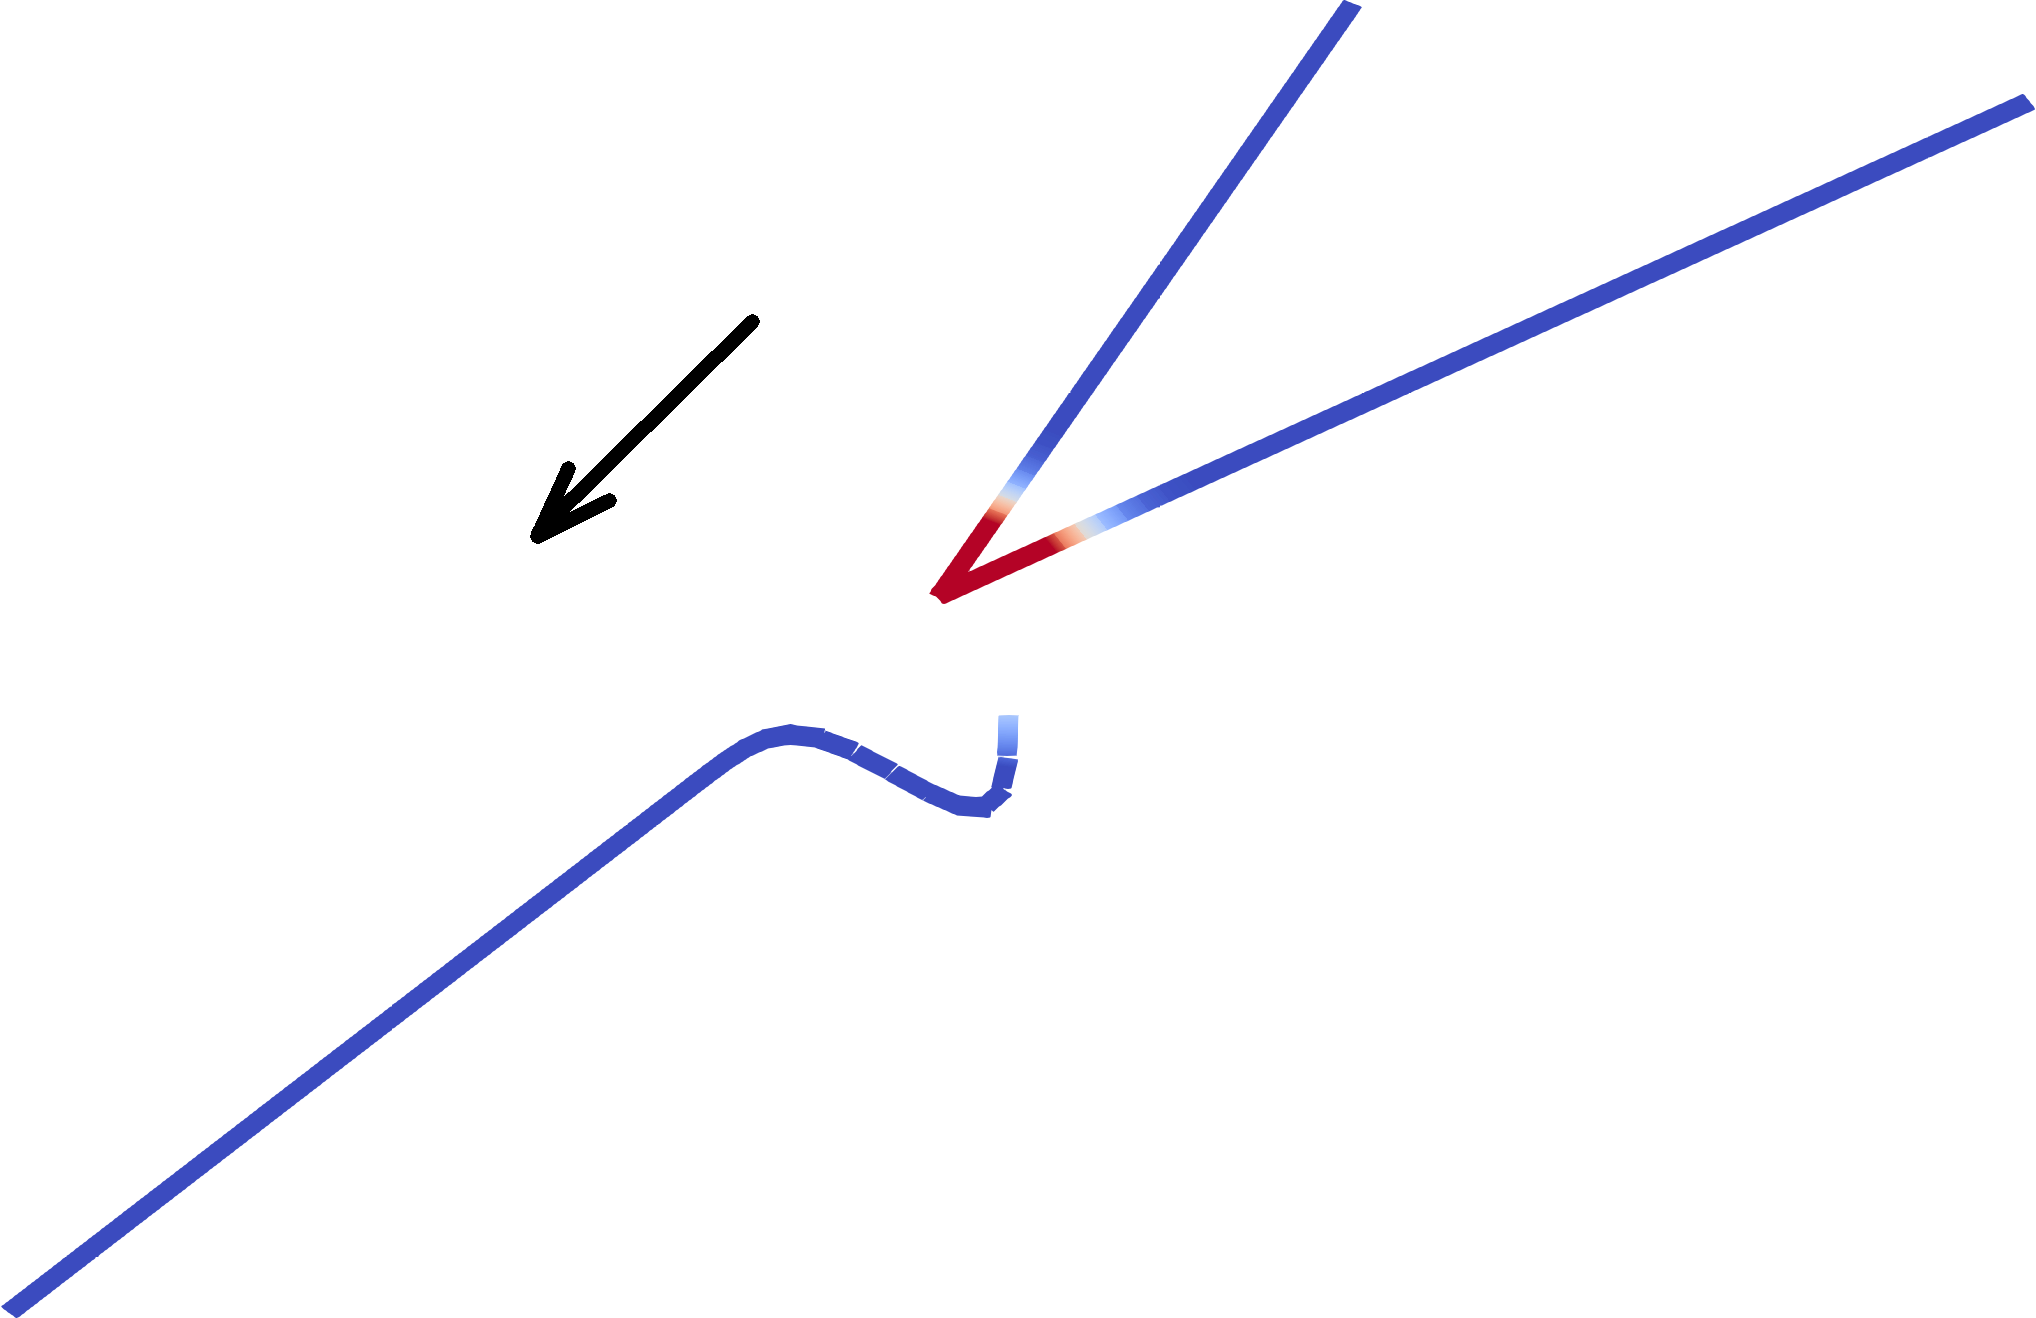
\includegraphics[width=0.4\linewidth]{prob4_time/w2_1.png}
\caption{$t = 0.22$}\label{fig:prob4_w12_b}
\end{subfigure}\\
\hfill \\
\hfill \\
\begin{subfigure}{1.0\linewidth}\centering
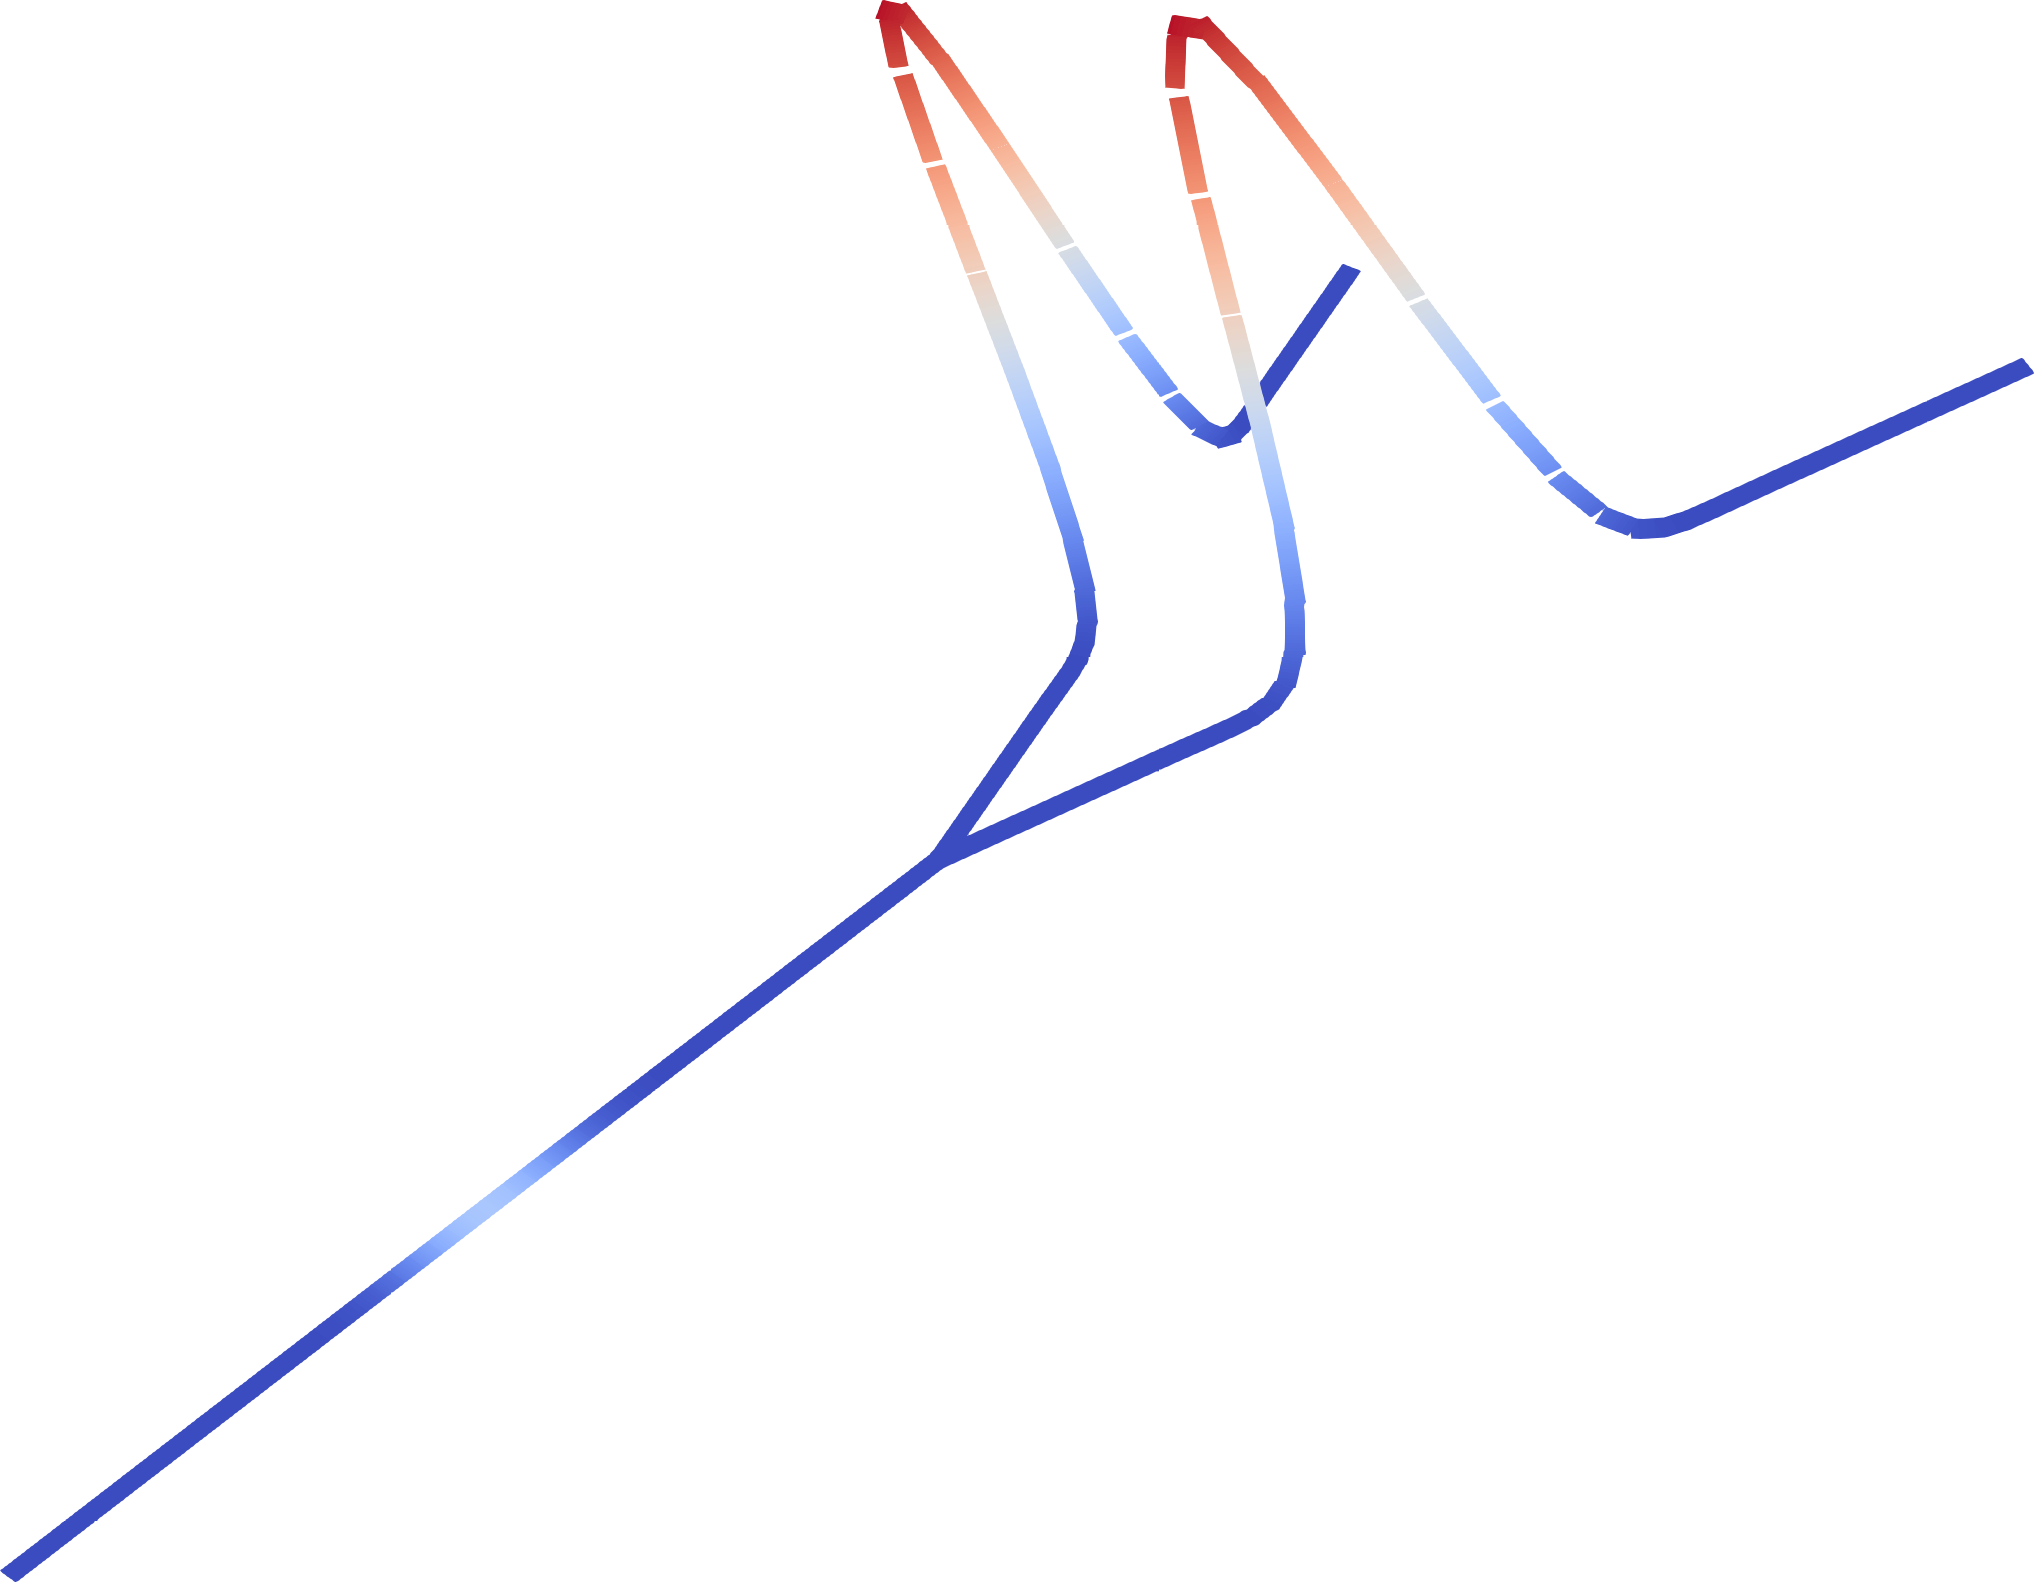
\includegraphics[width=0.4\linewidth]{prob4_time/w1_2.png}
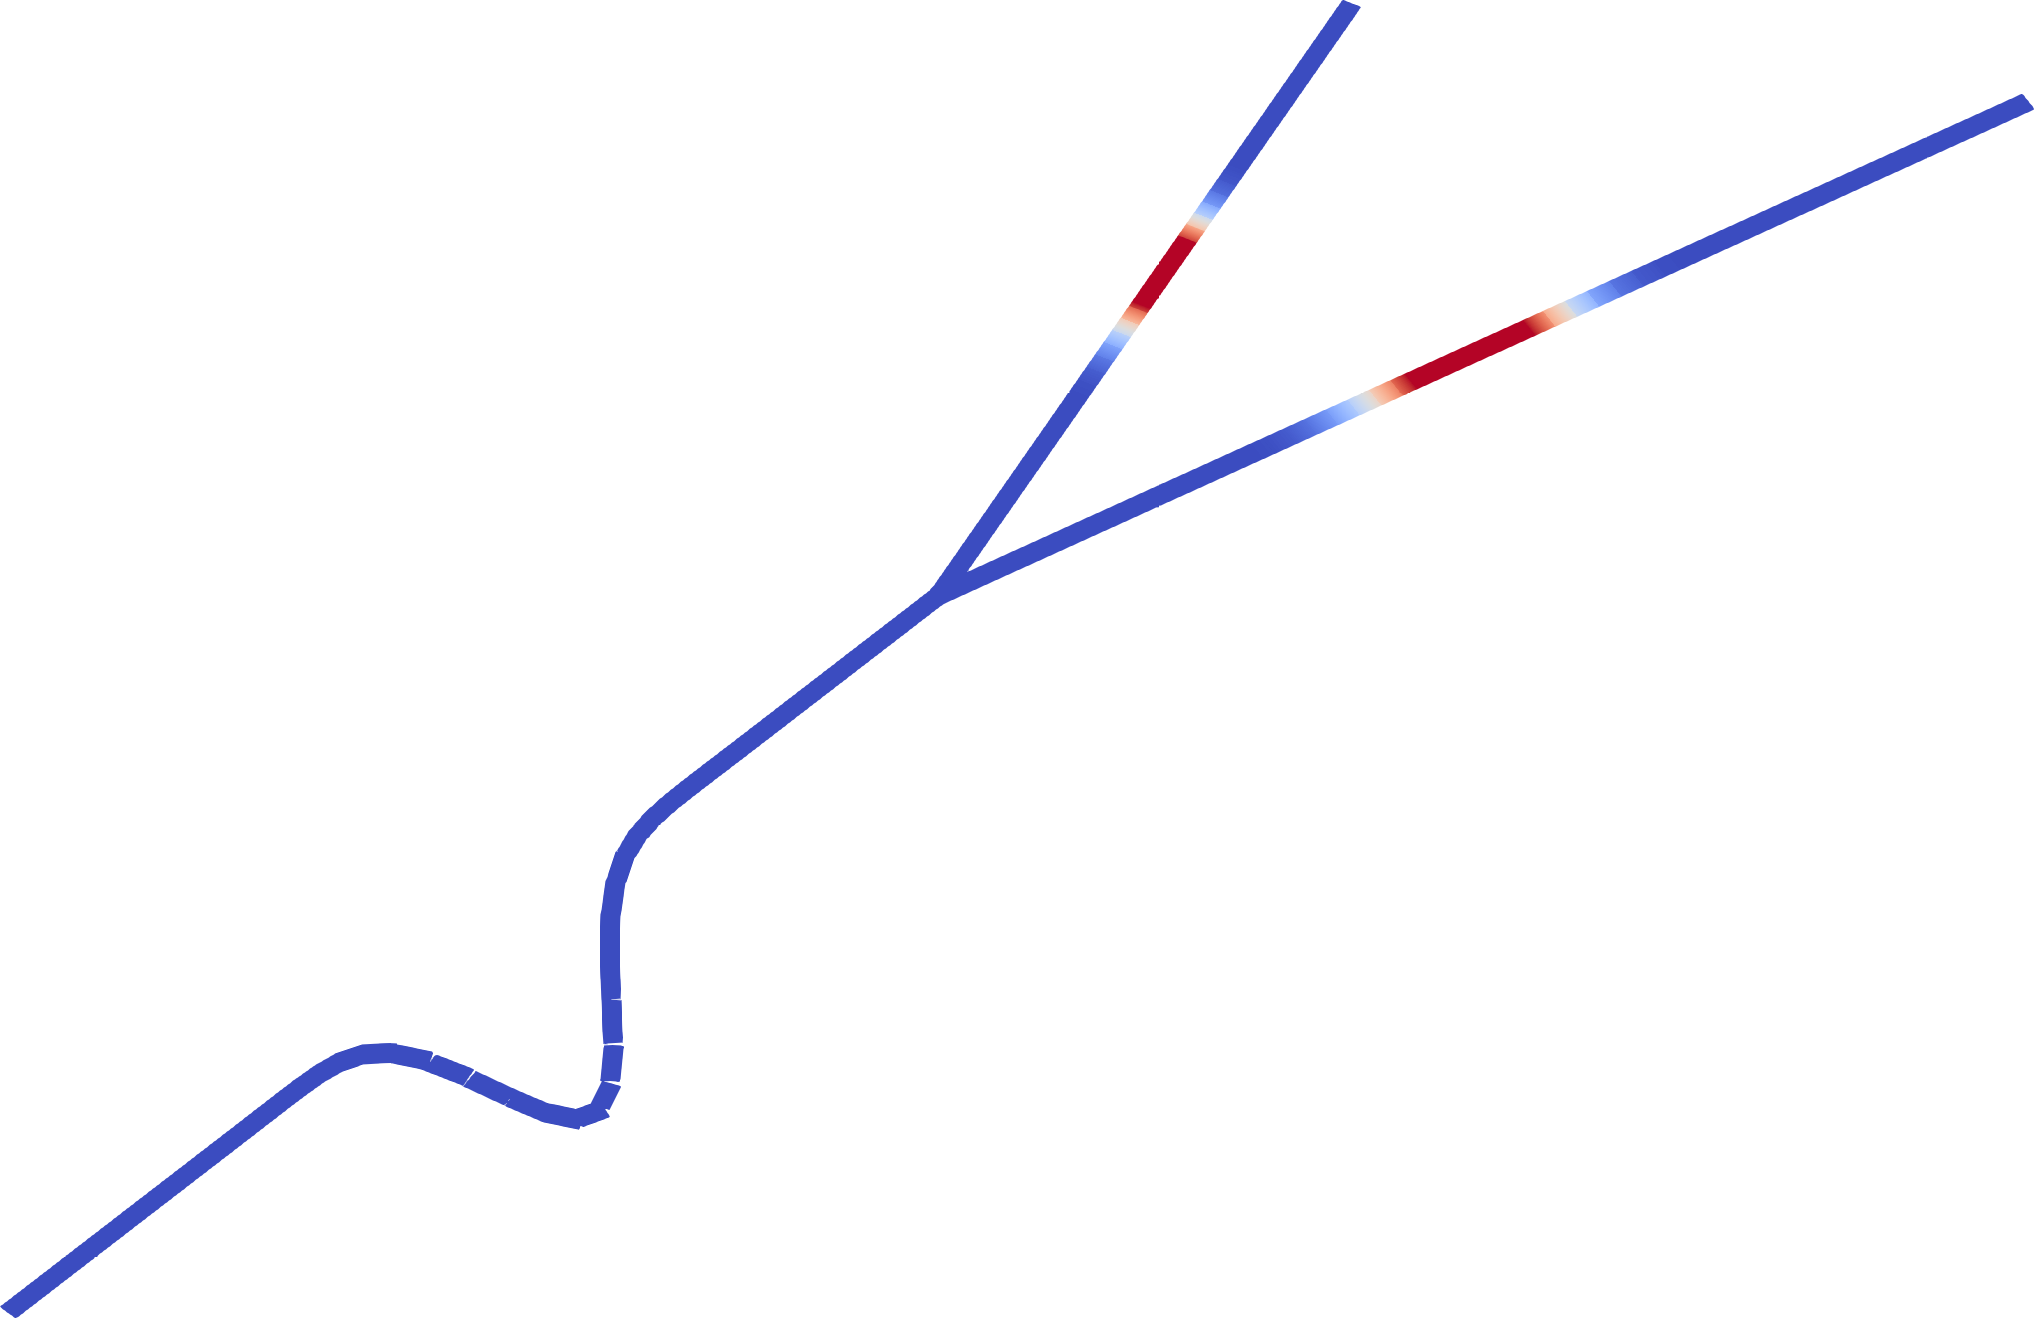
\includegraphics[width=0.4\linewidth]{prob4_time/w2_2.png}
\caption{$t=0.3$}\label{fig:prob4_w12_c}
\end{subfigure}\\
\caption{Значение переменной $w_1$ (слева) и $w_2$ (справа) на различные моменты времени}\label{fig:prob4_w12}
\end{figure}

В качестве граничного условия использовалось фиксированное входное значение
площади поперечного сечения $a = A$ и зависимость скорости от времени вида:
\begin{equation}
\nonumber
u_{in}(t) = 0.01\exp\left(-5000(t-0.05)^2\right).
\end{equation}
Таким образом, на вход подаётся единичная волна с пиковым
значением скорости $0.01$ м/с в момент времени $0.05$ с.

Расчёты проедены на сетке из 120 конечных элементов
(что соответствовало шагу по пространству $\dx = 0.005$ м)
с шагом по времени $\dt = 2.5\cdot10^{-4}$ с.
При выбранных параметрах сосудов скорость возмущений 
составляла $c_0=1.2$ м/с и $c_0 = 2.94$ м/с
для первого и вторых сосудов соответственно.
То есть число Куранта составляло $\CFL\approx0.15$.


Продвижение волны давления и скорости представлены на рис.~\ref{fig:prob4_pv}.
Поступательная волна повышенного давления и скорости
формируется от входного сечения (рис.~\ref{fig:prob4_pv_a})
и движется вперёд до точки разветвления (рис.~\ref{fig:prob4_pv_b}).
В этой точке происходит отражение части волны назад, после чего
наблюдаются уже две волны (рис.~\ref{fig:prob4_pv_c}):
поступательная волна продолжает движение по выходным сегментам графа,
а возвратная волна повышенного давления и пониженной (отрицательной)
скорости движется к входному сечению.

\begin{figure}[h!]
\begin{subfigure}{0.5\linewidth}\centering
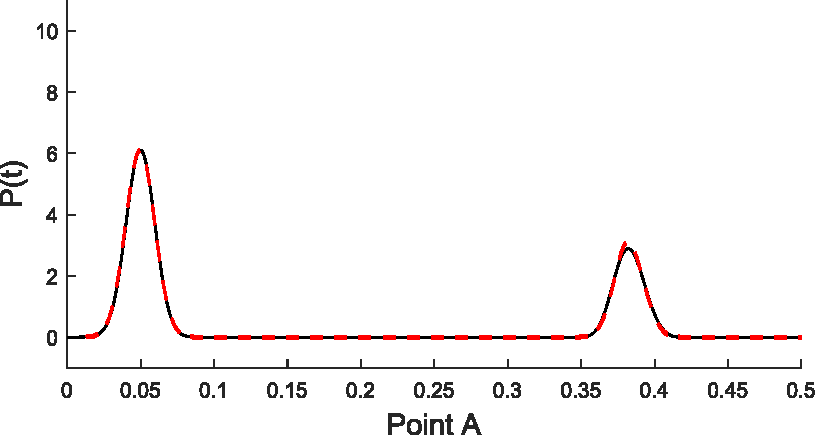
\includegraphics[width=0.9\linewidth]{problem4_pA1.pdf}
%\caption{}\label{fig:prob4_a}
\end{subfigure}%
\begin{subfigure}{0.5\linewidth}\centering
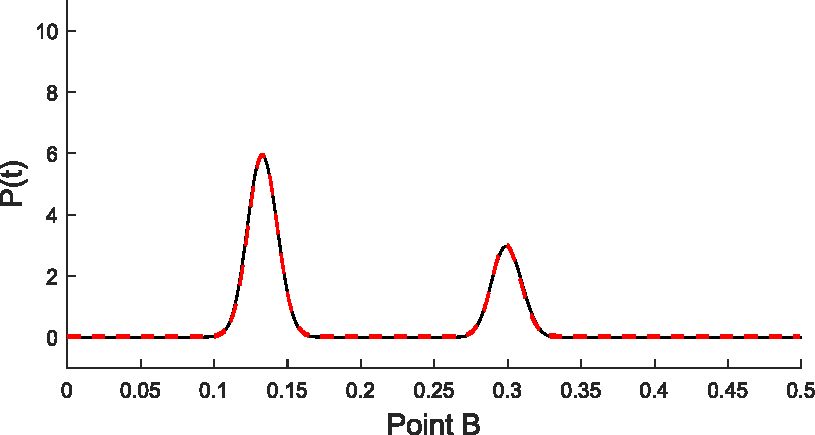
\includegraphics[width=0.9\linewidth]{problem4_pB1.pdf}
%\caption{}\label{fig:prob4_b}
\end{subfigure} \\
\hfill \\
\begin{subfigure}{0.5\linewidth}\centering
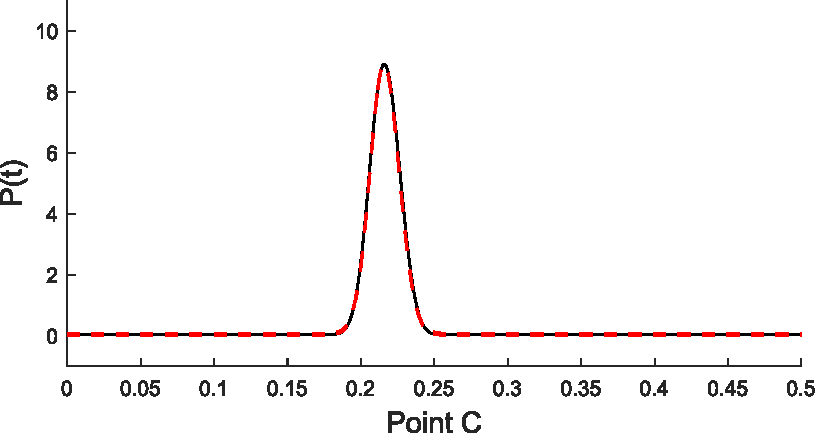
\includegraphics[width=0.9\linewidth]{problem4_pC1.pdf}
%\caption{}\label{fig:prob4_c}
\end{subfigure}%
\begin{subfigure}{0.5\linewidth}\centering
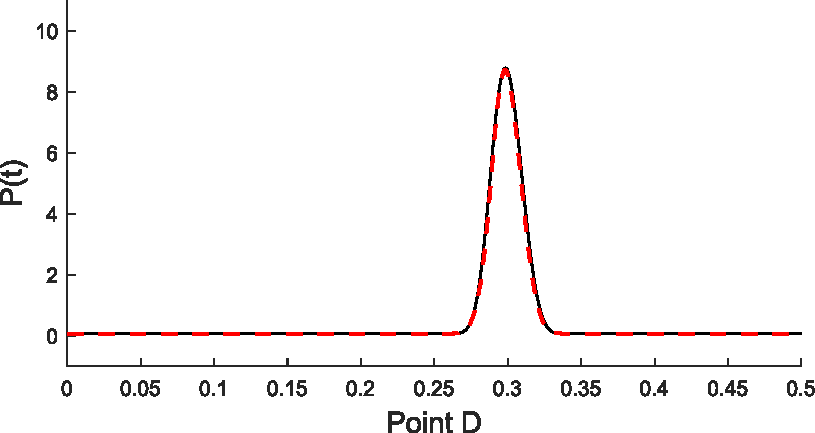
\includegraphics[width=0.9\linewidth]{problem4_pD1.pdf}
%\caption{}\label{fig:prob4_d}
\end{subfigure}\\
\hfill \\
\begin{subfigure}{0.5\linewidth}\centering
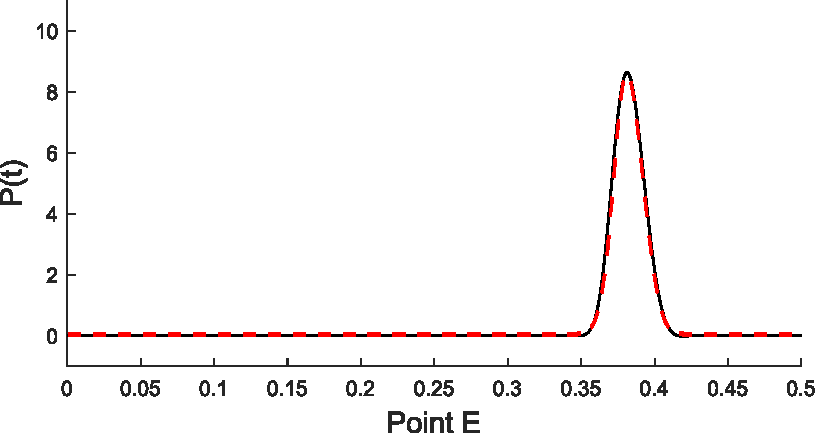
\includegraphics[width=0.9\linewidth]{problem4_pE1.pdf}
%\caption{}\label{fig:prob4_e}
\end{subfigure}%
\caption{Сравнение значения давления в контрольных точках. Сплошная линия -- наш расчёт, пунктирная -- результаты~\cite{Xiu:2007}}\label{fig:prob4_pt}
\end{figure}


Чтобы отделить поступательные волны от возвратных
был произведён пересчёт расчётных параметров
в переменные Римана $w_1$, $w_2$.
Их эволюция представлена на рис.~\ref{fig:prob4_w12}.
Как и следует из математического смысла этих переменных, каждая
из них содержит волны только одного направления.
Видно, что волна $w_2$ формируется
в момент, когда поступательная волна $w_1$
достигает точки разветвления (рис.~\ref{fig:prob4_w12_b}),
после чего волны $w_1$  и $w_2$ двигаются в противоположенных направлениях (рис.~\ref{fig:prob4_w12_c}).

Для сравнение полученных в результате наших расчётов данные с результатами из работы~\cite{Xiu:2007} 
были построены графики значения давления в контрольных точках (расположение контрольных точек смотри на рис.~\ref{fig:prob4_pv_a}).
Наложение графиков, демонстрирующее хорошее совпадение результатов, представлено на рис.~\ref{fig:prob4_pt}.
На графиках для точек A и B видно, что через соответствующие контрольные точки проходит
две волны. Сначала поступательная, потом отражённая возвратная.
Тут же следует отметить, что отсутствие других возмущений
говорит о корректной работе неотражающих граничных условий.


\subsection{Течение в системе сосудов}
Для иллюстрации применения численного метода
рассмотрим задачу о течении в системе из семи сосудов, представленных на рис.~\ref{fig:seven_vessel}.
\begin{figure}[h!]
\centering
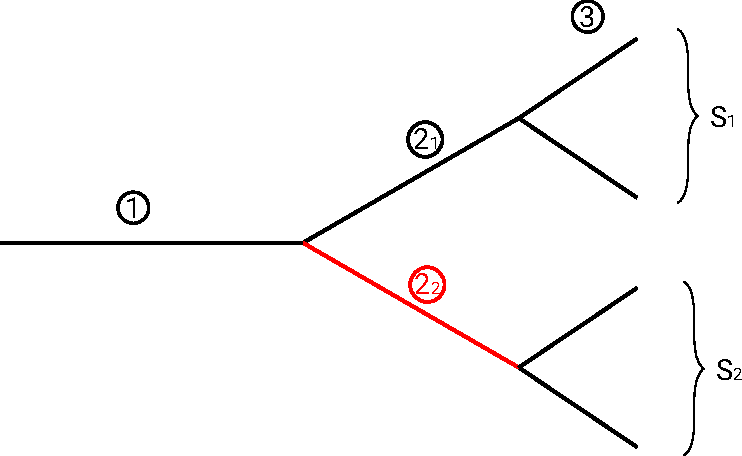
\includegraphics[width=0.6\linewidth]{seven_vessel.pdf}
\caption{Система из семи сосудов}\label{fig:seven_vessel}
\end{figure}%

Сосуды поделены на три группы: в группе $1$ один крупный сосуд,
 в группе $2$ два средних сосуда и в группе $3$ четыре малых сосуда.
Базовые свойства этих сосудов приведены в таблице \cref{tab:prob5_vessel}.

\begin{equation}
\label{tab:prob5_vessel}
\begin{array}{l|c|c|c}
\text{параметр}  & \text{сосуд 1} & \text{сосуды 2} & \text{сосуды 3}\\
\hline
\text{длина, м} & 1.0 & 0.8 & 0.5\\
\hline
R\text{, мм} & 5.0 & 4.0 & 3.0\\
\hline
E\text{, МПа} & \multicolumn{3}{c}{1.0}\\
\hline
h\text{, мм} & \multicolumn{3}{c}{0.15}\\
\hline
\rho\text{, кг/м\textsuperscript{3}} & \multicolumn{3}{c}{1050}\\
\hline
\mu\text{, Па с} & \multicolumn{3}{c}{0}\\
\hline
\end{array}
\end{equation}

Упругие свойства нижнего из промежуточных сосудов (обозначен $2.2$ на рисунке~\ref{fig:seven_vessel})
в зависимости от варианта расчёта изменяются согласно вариантам, представленным в таблице~\ref{tab:prob5_case}.
\begin{equation}
\label{tab:prob5_case}
\begin{array}{l|c|c|c|c}
\text{параметр}  & \text{вариант I} & \text{вариант II} & \text{вариант III} & \text{вариант IV}\\
\hline
R\text{, мм} & 4.0 & 4.0 & 4.0/\sqrt{2} & 4.0/\sqrt{2} \\
\hline
E\text{, МПа} & 1.0 & 10 & 1 & 10 \\
\hline
\end{array}
\end{equation}
Такие изменения характерны для склеротических поражений сосудов, при которых
увеличивается жёсткость стенки и уменьшается эффективный радиус сосуда.
Вариант I будем считать базовым, в варианте II увеличен модуль упругости сосуда,
в варианте III уменьшен радиус сосуда, вариант IV является суммой изменений из вариантов II и III.

На входе устанавливается периодическое значение расхода $q_{in}(t)$
с максимальным значением в $20$мл/сек:
\begin{equation*}
q_{in}(t) = 2\cdot10^{-5}\max(0, \sin(2\pi t / T)).
\end{equation*}
Рассматривались два периода $T$, соответствующие частоте сердцебиения \gls{bpm} в 60 (спокойный пульс) и 180 (высокий пульс) ударов в минуту.
В качестве выходного параметра мониторятся выходное значение расхода в сечениях, обозначенных на рис.~\ref{fig:seven_vessel} как $S_1$ (неповрежденная сторона системы)
и $S_2$ (повреждённая сторона системы).

Результаты для значения $bpm=60$ приведены на рис.~\ref{fig:prob5_q1}, а для $bpm=180$ -- на рис.~\ref{fig:prob5_q2}.
На рис.~\ref{fig:prob5_time} приведено значение скорости течения на различные моменты времени.
Видно, что оба типа повреждения значительно уменьшают количество
жидкости, протекающей через повреждённую сторону, при этом также происходит
изменения величины расхода и для неповреждённой стороны. В частности, там наблюдаются потоки, текущие в обратном направлении ($u<0$).
Для $bpm=180$ качественная картина не меняется, но при этом перепады значений расходов между сечениями $S_1$ и $S_2$
кратно увеличивается.
Из этого можно сделать вывод, что негативные последствия, связанные с нарушением эластичности стенок сосудов, проявляет себя сильнее при
высоком пульсе.

\begin{figure}[h!]
\begin{subfigure}{0.5\linewidth}\centering
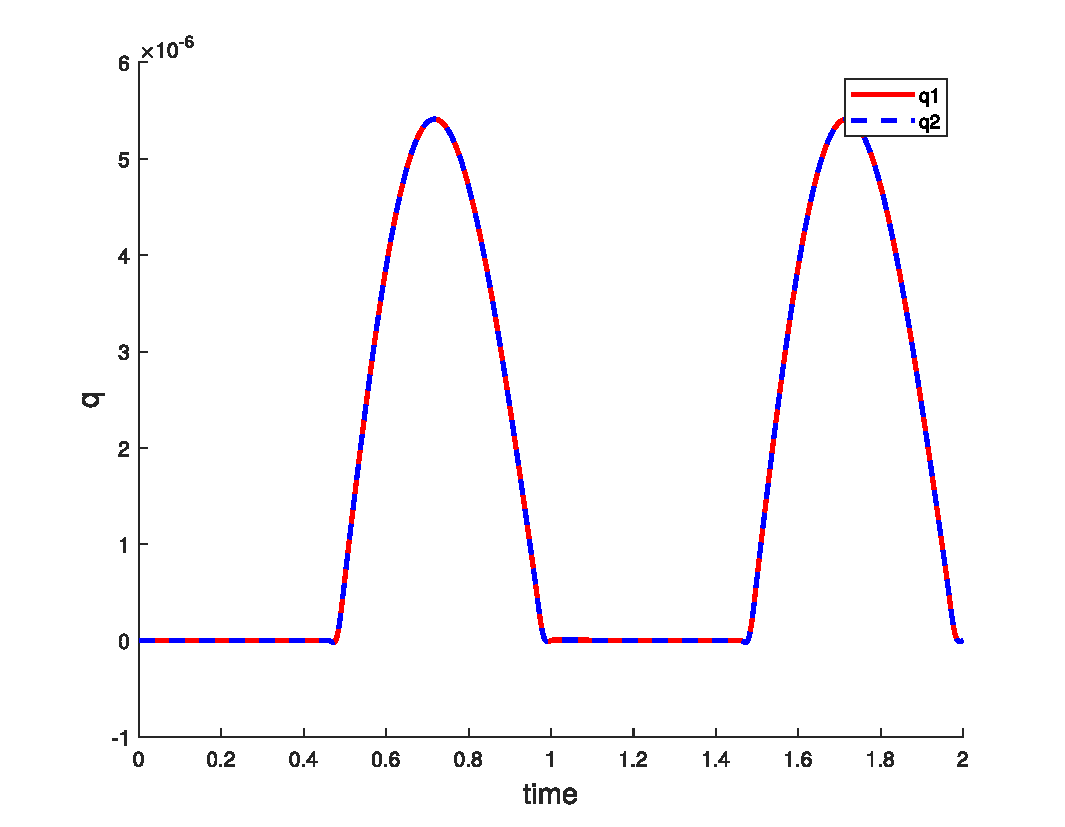
\includegraphics[width=0.9\linewidth]{q1_eq.pdf}
\caption{Вариант I}\label{fig:prob5_q1_eq}
\end{subfigure}%
\begin{subfigure}{0.5\linewidth}\centering
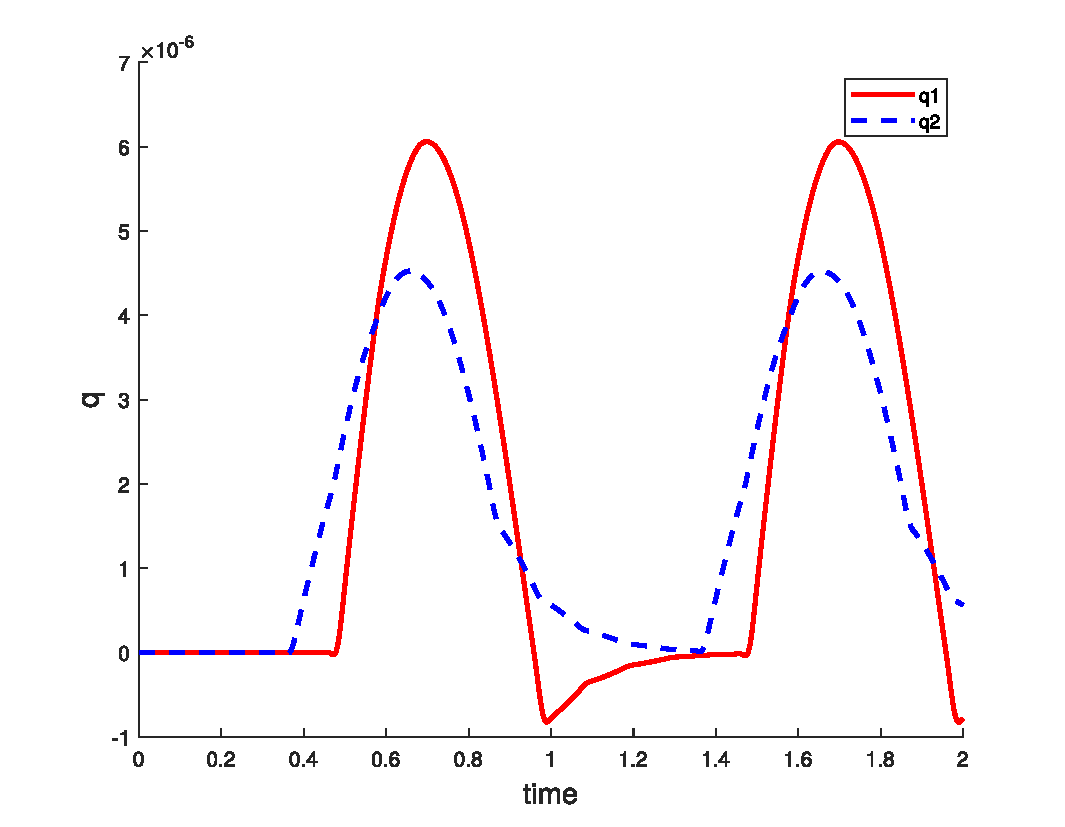
\includegraphics[width=0.9\linewidth]{q1_e10.pdf}
\caption{Вариант II}\label{fig:prob5_q1_e10}
\end{subfigure} \\
\hfill \\
\begin{subfigure}{0.5\linewidth}\centering
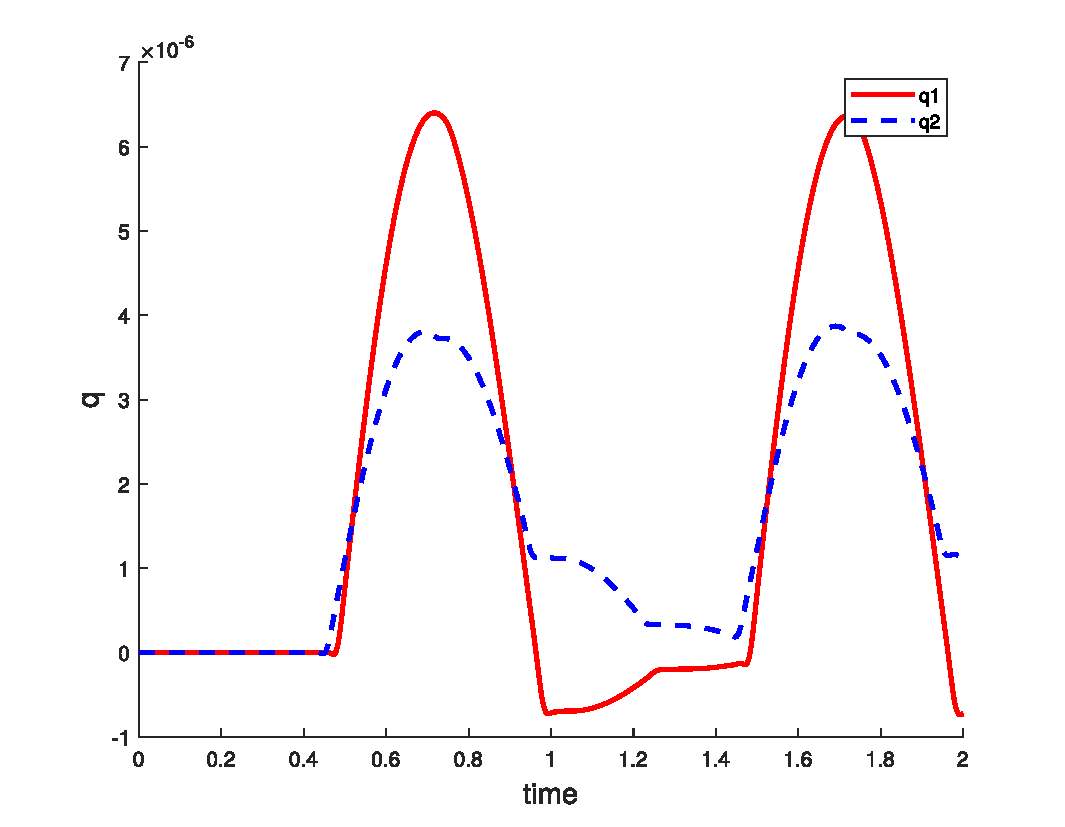
\includegraphics[width=0.9\linewidth]{q1_a2.pdf}
\caption{Вариант III}\label{fig:prob5_q1_a2}
\end{subfigure}%
\begin{subfigure}{0.5\linewidth}\centering
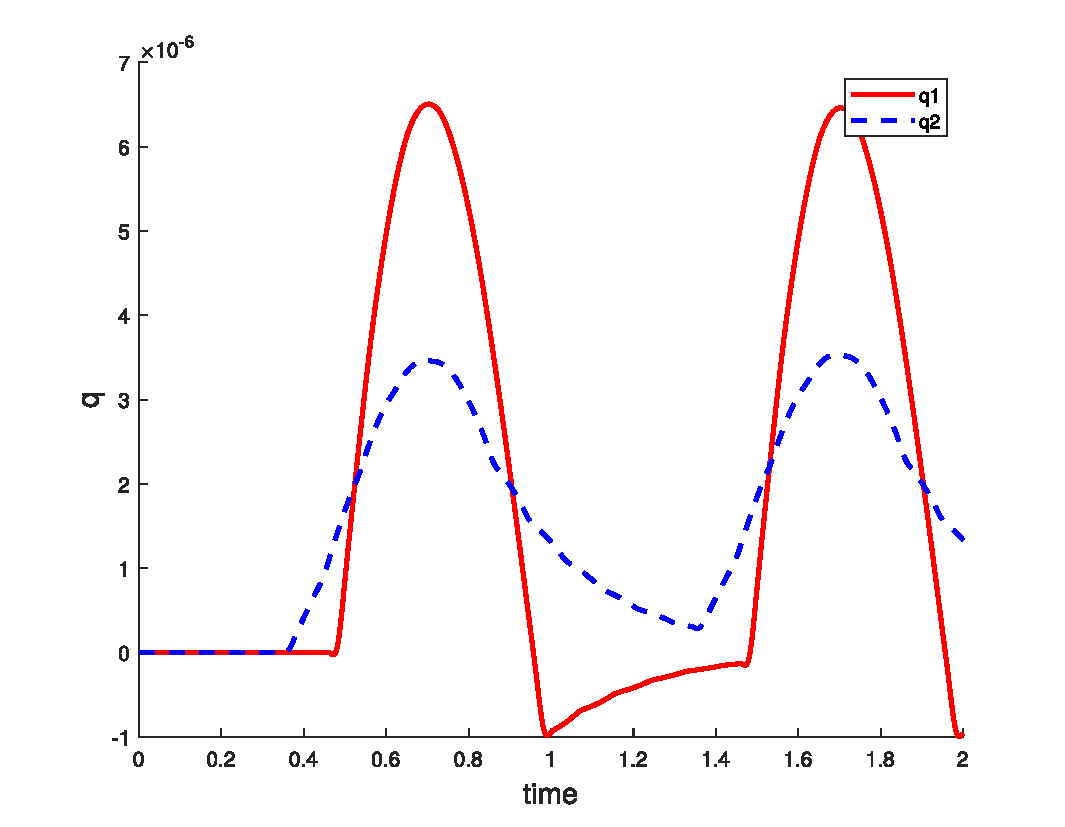
\includegraphics[width=0.9\linewidth]{q1_e10a2.pdf}
\caption{Вариант IV}\label{fig:prob5_a1_e10a2}
\end{subfigure}%
\caption{Значение расходов через сечения $S_1$ (красная линия) и $S_2$ (синяя линия) для различных способов повреждения сосудов, ведущих к $S_2$. Частота -- $bpm=60$}
\label{fig:prob5_q1}
\end{figure}

\begin{figure}[h!]
\begin{subfigure}{0.5\linewidth}\centering
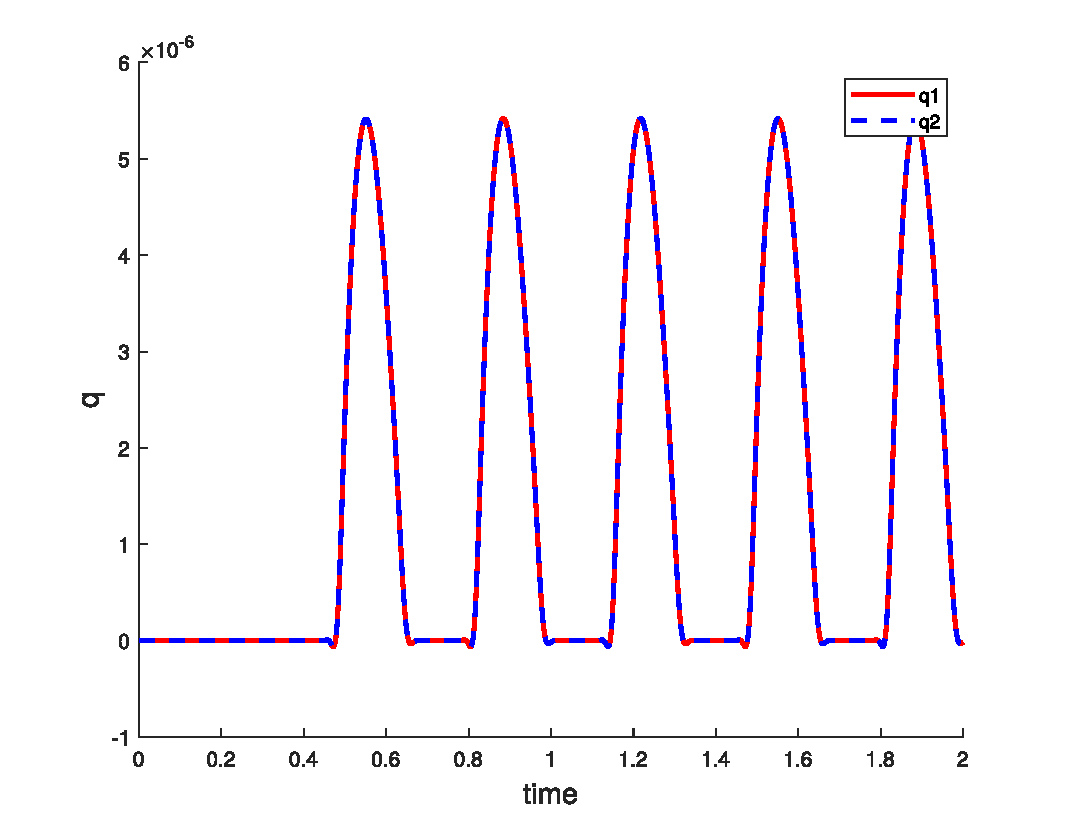
\includegraphics[width=0.9\linewidth]{q2_eq.pdf}
\caption{Вариант I}\label{fig:prob5_q2_eq}
\end{subfigure}%
\begin{subfigure}{0.5\linewidth}\centering
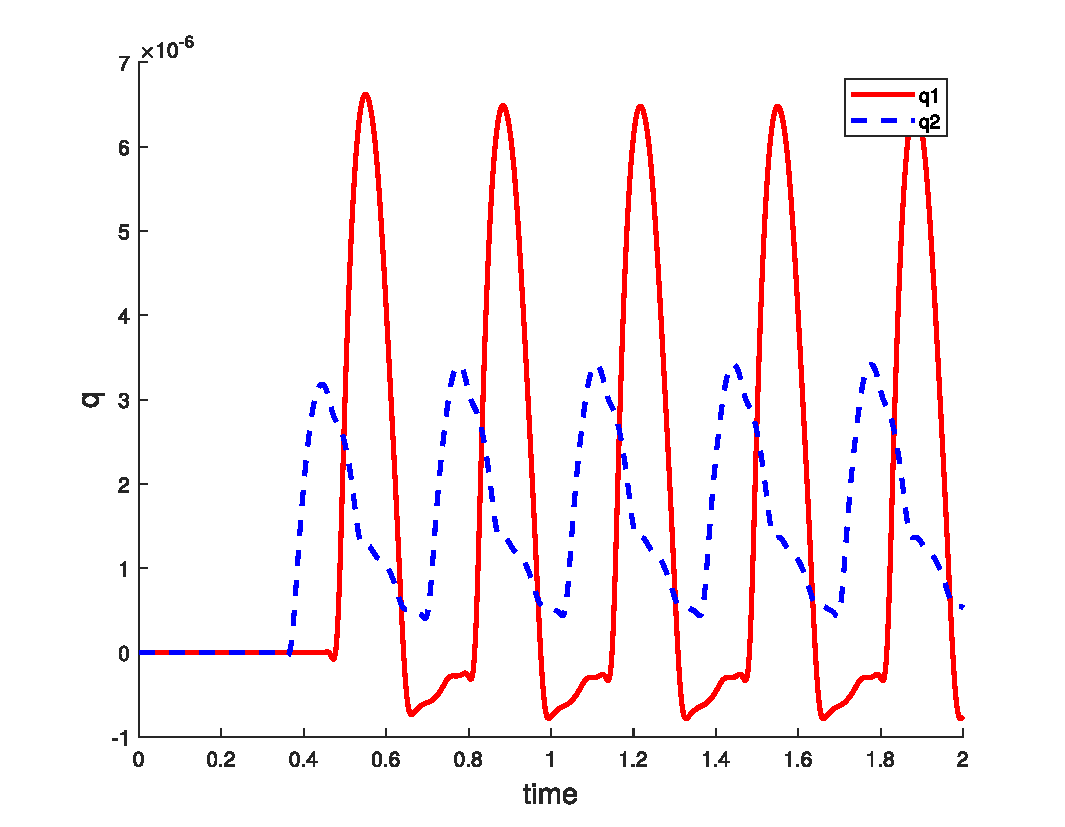
\includegraphics[width=0.9\linewidth]{q2_e10.pdf}
\caption{Вариант II}\label{fig:prob5_q2_e10}
\end{subfigure} \\
\hfill \\
\begin{subfigure}{0.5\linewidth}\centering
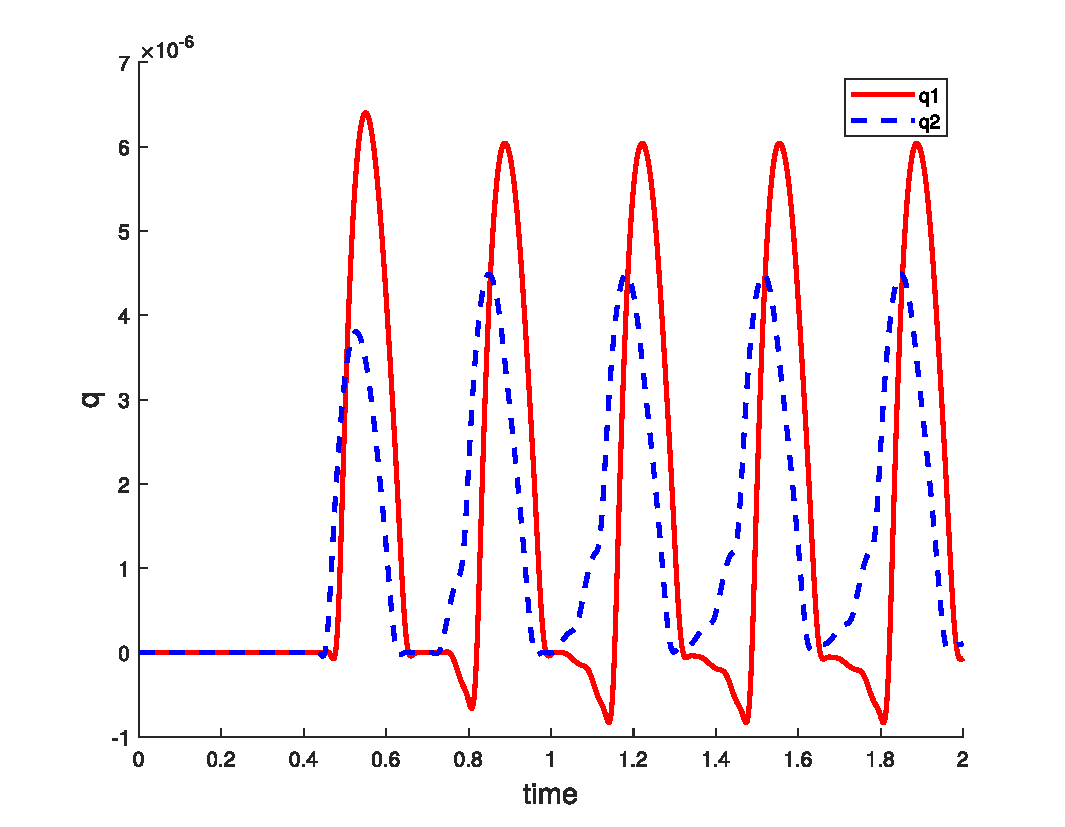
\includegraphics[width=0.9\linewidth]{q2_a2.pdf}
\caption{Вариант III}\label{fig:prob5_q2_a2}
\end{subfigure}%
\begin{subfigure}{0.5\linewidth}\centering
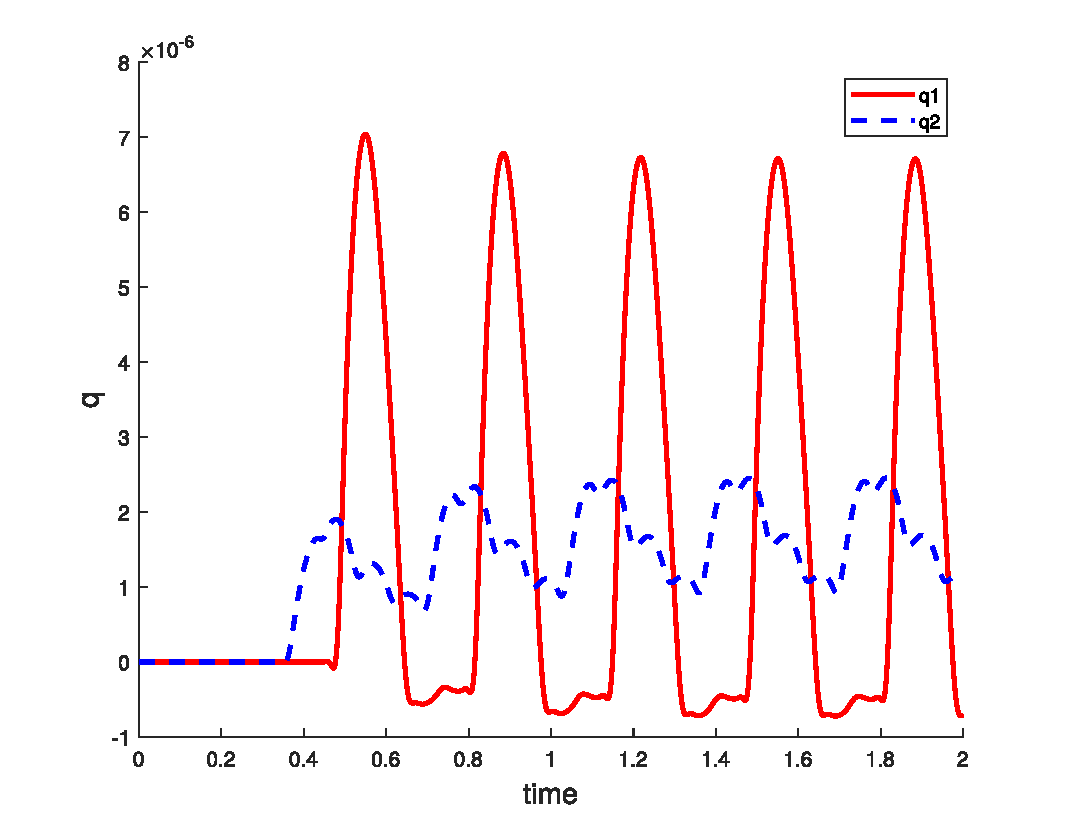
\includegraphics[width=0.9\linewidth]{q2_e10a2.pdf}
\caption{Вариант IV}\label{fig:prob5_a2_e10a2}
\end{subfigure}%
\caption{Значение расходов через сечения $S_1$ (красная линия) и $S_2$ (синяя линия) для различных способов повреждения сосудов, ведущих к $S_2$. Частота -- $bpm=180$}
\label{fig:prob5_q2}
\end{figure}

\begin{figure}[h!]
\centering
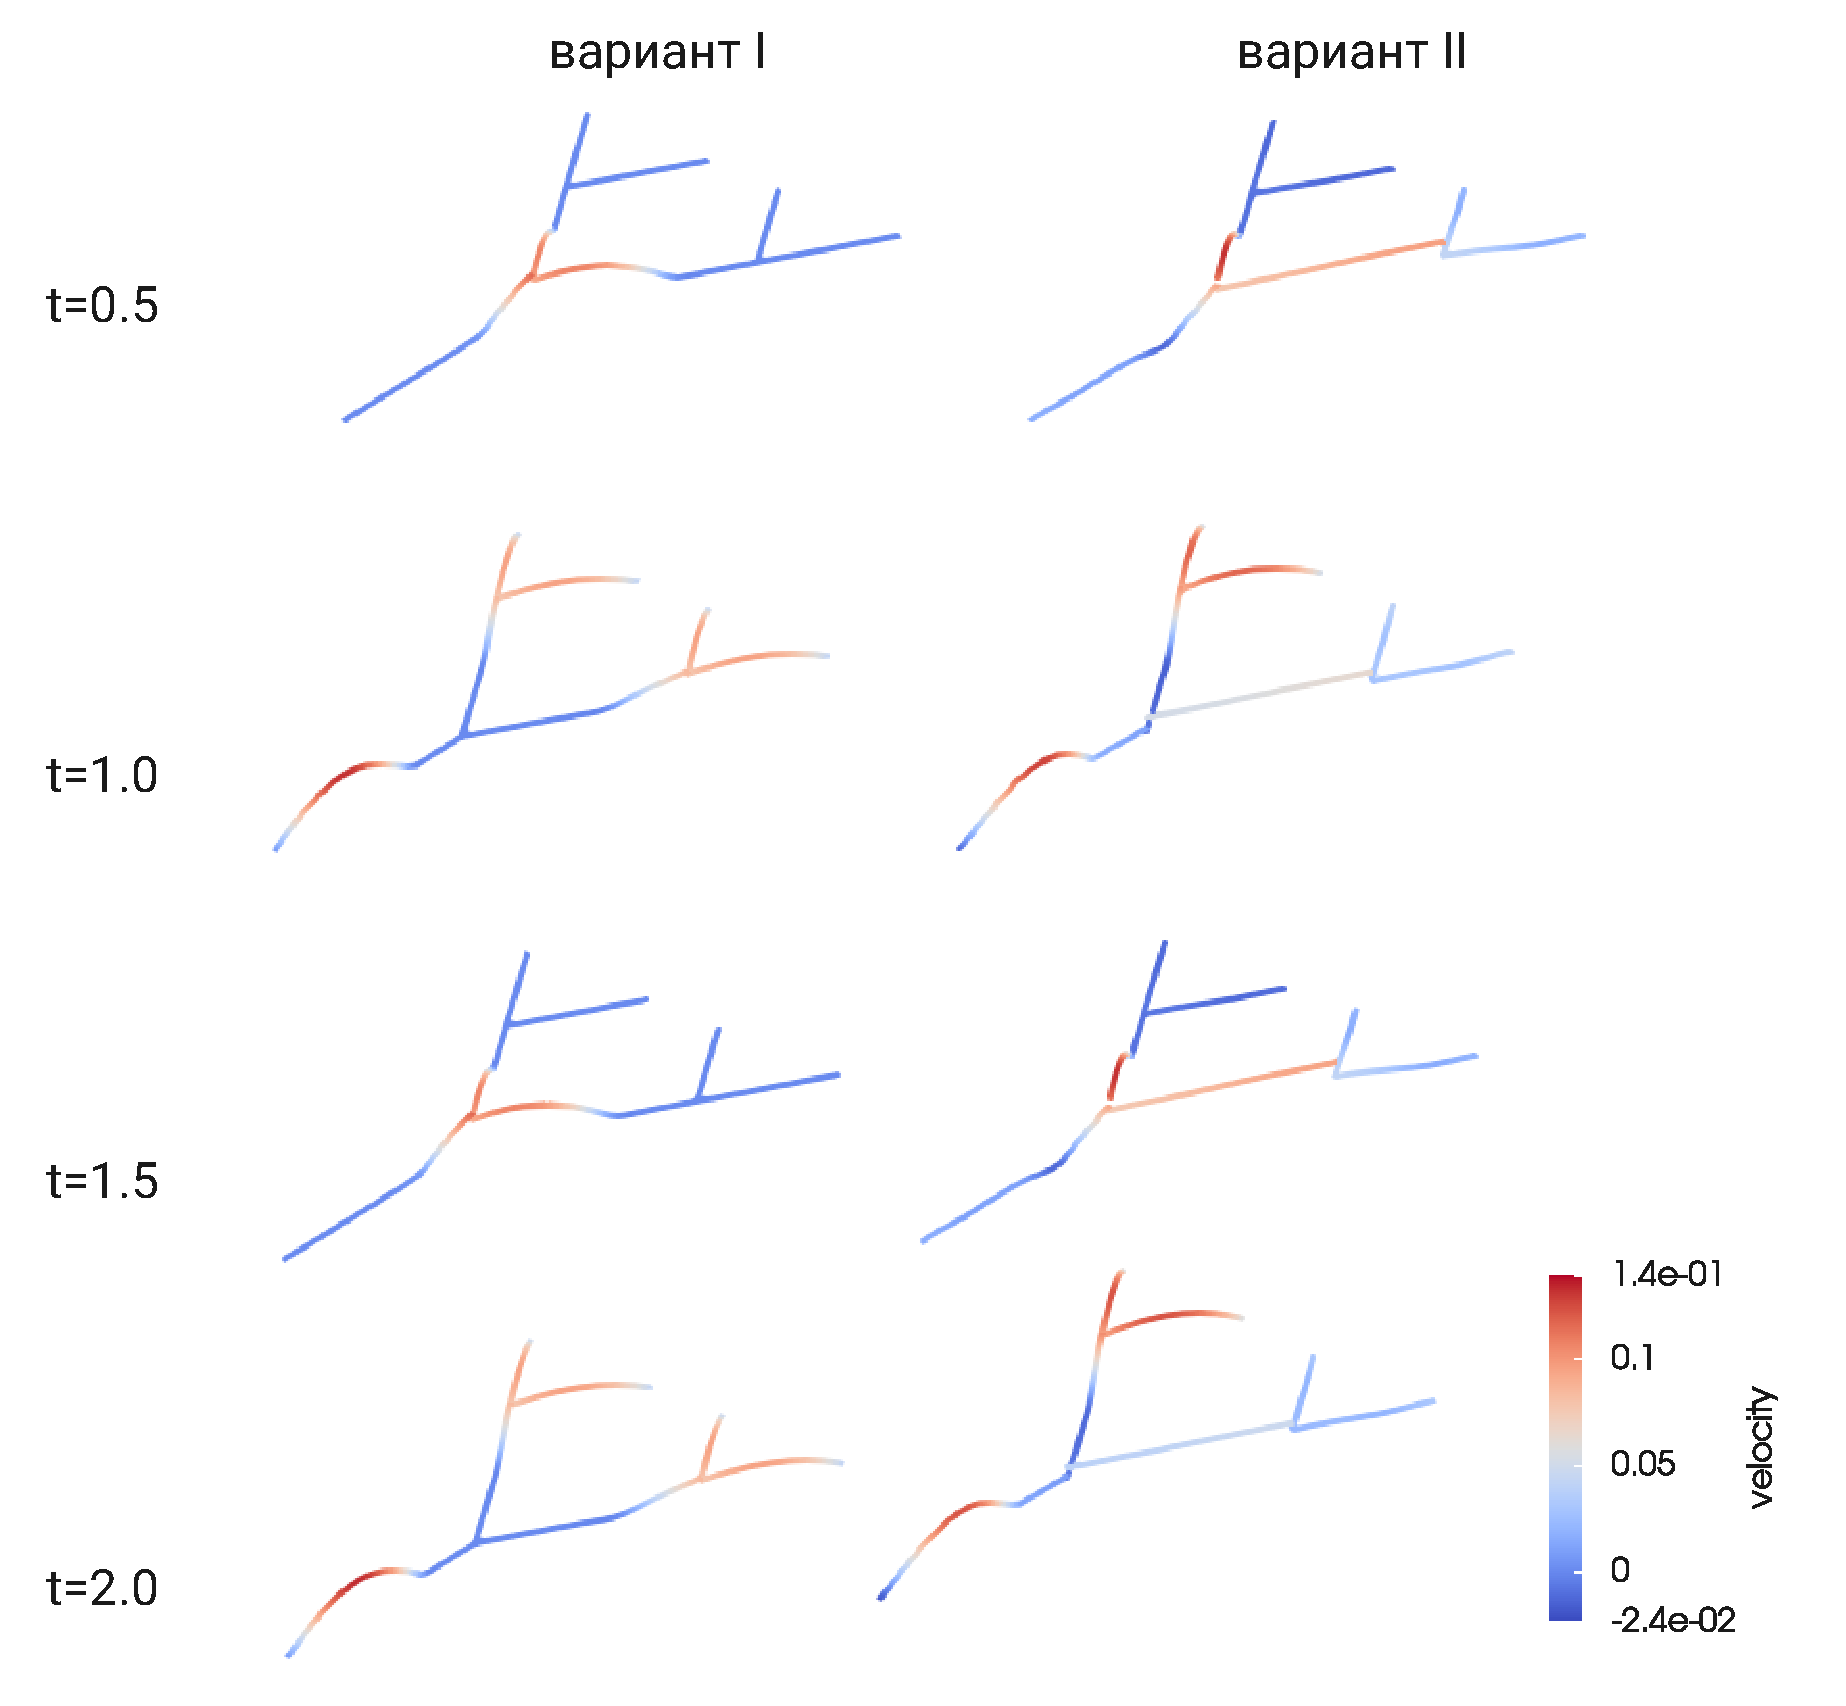
\includegraphics[width=1.0\linewidth]{problem5_time.pdf}
\caption{Значение скорости течения $u$ на различные моменты времени при частоте $bpm=180$. Слева вариант I, справа вариант IV}\label{fig:prob5_time}

\end{figure}
